%% ============================================================
%%  RTX PRO 6000 Blackwell 推理性能综述
%%  NeurIPS 风格双栏排版（单栏摘要 + 双栏正文）
%%
%%  这是 PAPER.md 的一种渲染，不承载任何新事实。
%%  事实源仍是 PAPER.md，它由 check_paper.py / audit_paper.py 校验。
%%  本文件只负责排版。
%%
%%  编译：xelatex main.tex  （两遍，交叉引用才正确）
%% ============================================================
\documentclass[10pt,twocolumn]{article}

%% ---------- 中文支持 ----------
\usepackage[UTF8,fontset=none]{ctex}

%% 字体：正文宋体，标题黑体，等宽用 Consolas。
%% ⚠️ 中文论文的正文一律用宋体（衬线），标题用黑体（无衬线），
%% 这是国内学术排版的通行规范；把正文排成无衬线会显著降低长时间阅读的舒适度。
%% ⚠️ 楷体的族名是 KaiTi，不是 SimKai —— 写错会让 fontspec 报 nullfont，
%% 而报错信息（Cannot use \XeTeXOTfeaturetag with nullfont）完全指不出是哪个字体。
\setCJKmainfont{SimSun}[BoldFont=SimHei,ItalicFont=KaiTi]
%% ⚠️ SimHei 没有独立的粗体字形，不声明会报「Font shape undefined」，
%% 且 \textbf{} 里实际仍是细体 —— 视觉上粗体失效，而日志只是警告。
%% AutoFakeBold 用仿粗体补齐，这是中文排版里常见且可接受的折中。
\setCJKsansfont{SimHei}[BoldFont=SimHei,AutoFakeBold=1.2]
\setCJKmonofont{SimHei}
\setmainfont{Times New Roman}
%% ⚠️ 原文大量使用 ⭐ 🔥 ⚠️ 这类符号作强调标记，而 SimSun 没有这些字形，
%% 不指定回退就会在 PDF 上留空白或方框（且不报错）。
%% 用 Segoe UI Symbol 兜底：覆盖这些符号，且是**单色**符号字体。
%% ⚠️ 不能用 Segoe UI Emoji —— 彩色字体在 XeLaTeX 里会渲染成空白或黑块。
\newfontfamily\symfont{Segoe UI Symbol}[AutoFakeBold=1.2]
\newcommand{\sym}[1]{{\symfont #1}}
\setsansfont{Arial}
\setmonofont{Consolas}

%% ---------- 版面 ----------
\usepackage[a4paper,margin=2.05cm,columnsep=0.72cm]{geometry}
\usepackage{amsmath,amssymb}
\usepackage{graphicx}
\usepackage{booktabs}
\usepackage{tabularx,array,longtable,multirow}
\usepackage{caption}
\usepackage{enumitem}
\usepackage{titlesec}
\usepackage{xcolor}
\usepackage{fancyhdr}
\usepackage[hidelinks]{hyperref}
\usepackage{cleveref}
\usepackage{microtype}
\usepackage{listings}
%% 代码块：开自动折行，否则双栏里长命令行会溢出（实测 132pt）。
\lstset{
  basicstyle=\ttfamily\scriptsize,
  breaklines=true,
  breakatwhitespace=false,
  columns=fullflexible,
  frame=none,
  xleftmargin=0.6em,
  aboveskip=4pt,
  belowskip=4pt
}

%% 图表标题：小号、居中、题注与图体间距收紧。
%% 默认间距在双栏里会把图挤到下一页，收紧后版面利用率明显提高。
\captionsetup{
  font=small,
  labelfont=bf,
  labelsep=quad,
  skip=4pt,
  justification=centering
}
\captionsetup[table]{position=top}

%% 断行容差：中文没有空格，断行点比英文稀疏，默认容差下 LaTeX
%% 宁可溢出也不肯拉开字距。三处一起放宽：
%%   tolerances 放宽断行代价上限；
%%   emergencystretch 给它额外的可拉伸量（关键时刻允许某行稍松）；
%%   XeTeX 的 CJK 断行还需要把标点挤压算进去，故 sloppy 也开。
%% ⚠️ 只加 \sloppy 会让所有行都变松，故只加 emergencystretch + 容差。
\setlength{\emergencystretch}{3em}
\tolerance=2000
\hbadness=2000
\hyphenpenalty=50

%% 标题层级：中文论文习惯章标题较大、节标题次之，且都留白充足。
\titleformat{\section}{\large\bfseries\sffamily}{\thesection}{0.6em}{}
\titleformat{\subsection}{\normalsize\bfseries\sffamily}{\thesubsection}{0.5em}{}
\titleformat{\subsubsection}{\normalsize\bfseries}{\thesubsubsection}{0.4em}{}
\titlespacing*{\section}{0pt}{10pt plus 2pt minus 2pt}{5pt plus 1pt}
\titlespacing*{\subsection}{0pt}{7pt plus 1pt minus 1pt}{3pt plus 1pt}
\titlespacing*{\subsubsection}{0pt}{5pt plus 1pt minus 1pt}{2pt}

%% 列表：中文行距下默认间距偏大，收紧。
\setlist[itemize]{topsep=2pt,itemsep=1pt,parsep=0pt,leftmargin=1.4em}
\setlist[enumerate]{topsep=2pt,itemsep=1pt,parsep=0pt,leftmargin=1.6em}

%% 行距：中文正文 1.28 倍较接近「单倍半」的观感，
%% 既不像 LaTeX 默认那样挤，也不会松散到浪费版面。
\linespread{1.28}
\setlength{\parskip}{3.2pt plus 1pt}
\setlength{\parindent}{1.6em}

%% 页眉页脚：双栏论文通常只保留页码。
\pagestyle{fancy}
\fancyhf{}
\renewcommand{\headrulewidth}{0pt}
\fancyfoot[C]{\small\thepage}

%% 图表浮动体放宽：双栏下默认只允许很少的浮动体，容易全部堆到文末。
\renewcommand{\topfraction}{0.92}
\renewcommand{\bottomfraction}{0.85}
\renewcommand{\textfraction}{0.08}
\renewcommand{\floatpagefraction}{0.80}
\setcounter{topnumber}{4}
\setcounter{bottomnumber}{3}
\setcounter{totalnumber}{8}

\begin{document}

%% ---------- 标题区（单栏，跨通栏） ----------
%% ⚠️ 这里只放「主标题 + 副标题」——那是版式。
%% 数据快照 / 证据等级 / SKU 约定 三行属于**内容**（数字会失效），
%% 由 body.tex 开头那个 quote 块承载，不在这里写死，否则两处会各自漂移。
\twocolumn[{
\begin{center}
{\LARGE\bfseries\sffamily RTX PRO 6000 Blackwell 的推理性能\par}
\vspace{3pt}
{\large\sffamily 一次以证据等级为准的综述\par}
\end{center}
\vspace{6pt}
}]


\begin{quote}\small
\textbf{数据快照}：2026-10-29 ｜ \textbf{来源}：447 ｜ \textbf{证据}：3,002 ｜ \textbf{主张}：2,238

\textbf{全文证据等级}：所有数值最高为 \textbf{测量级（measured）}，无一条达到 \textbf{复现级（reproduced）} 或 \textbf{发布级（released）}。

\textbf{\sym{⚠}{} 全文 SKU 约定}：\texttt{WS} = Workstation Edition（600 W 主动散热）、\texttt{MQ} = Max-Q Workstation Edition（300 W）、\texttt{SE} = Server Edition（被动散热）。\textbf{凡来源未指明 SKU 的，标为「未指明」，不得当作三个 SKU 中的任何一个。}

\end{quote}


\begin{abstract}

本文综述 NVIDIA RTX PRO 6000 Blackwell（GB202，96 GB GDDR7，\texttt{sm\_120a}）在本地大模型推理上的性能表现，并与 RTX 5090、RTX 4090、RTX 6000 Ada 及数据中心加速器对照。我们不按「谁更快」组织材料，而按「这个数字能证明什么」组织。


\textbf{核心发现有八。}


\textbf{第一，预填与解码是两条曲线，差 110 倍，故「这张卡多快」本身有歧义。}同一张卡、同一个模型、同一套 llama.cpp 单流测量：预填 \textbf{4,757 tok/s}，解码 \textbf{43.16 tok/s}。预填瓶颈是算力，解码瓶颈是带宽，两者对硬件的要求几乎正交。三条证据互相印证：同带宽的 RTX 5090 解码持平；功耗从 300 W 翻到 600 W只让预填快约两成、解码几乎不动；互连（PCIe 对 NVLink）只在解码上拉开 66\%。故\textbf{长提示短回答时它是很快的卡，短提示长回答时它是最弱的一维。}而\textbf{首字延迟是第三个维度，与上面两个都不同步}：同一对卡开 EP 让首字从18,355 毫秒降到 673 毫秒（27 倍），吞吐只涨 2.3 倍、TPOT 几乎不变；而 2 张 B200 靠 NVLink 把吞吐做到高 1.66 倍、TPOT 做到低 2.3 倍，首字却是这张卡的 3.7 倍。


\textbf{第二，这个产品名不是一个配置，而是三个。} 同一名字下有 600 W 的 Workstation Edition、300 W 的 Max-Q、以及被动散热的 Server Edition。它们在同一模型同一命令下的解码吞吐差 \textbf{12.9\%-\hspace{0pt}13.1\%}；在同一功耗点（300 W）上 Server 版比 WS 版快 \textbf{38\%}。故「RTX PRO 6000 的 tok/s 是多少」这个问法本身需要先回答「哪个 SKU」。


\textbf{第三，容量不构成约束时，这张卡与消费级旗舰几乎打平。} UL Procyon 四模型文本生成中，WS 版相对 RTX 5090 的 token 速率优势只有 \textbf{1.5\%-\hspace{0pt}5.9\%}；而同一测试的总分差距达 \textbf{8\%-\hspace{0pt}18\%}。同一个测试的两个输出给出两种图景。


\textbf{第四，真正的差距出现在容量成为约束的边界上。} RTX 5090 无法加载 120B 模型，而这个系列以 \textbf{163.15 tok/s} 完成 GPT-OSS 120B；Llama 3.3 70B 上差距达 \textbf{928\%}。但这个百分比不是「更快」，而是「对方跑不了」。


\textbf{第五，与上代专业卡比，同一张卡有六个倍率，从 1.09 到 21.3，而它们都不假。}对 L40 Ada，多基准实测中位加速比 \textbf{1.09 倍}、胜率 78\%、最差 0.85 倍、最好 1.67 倍；而厂商宣称最高 \textbf{5.6 倍}（Llama 3 70B 单点口径）。\textbf{0.85 与 5.6 是同一对显卡。}规格上 L2 缓存相对 RTX A6000 是 21.3 倍，而对推理的意义接近于零。渲染则不同：SPECviewperf 15 中位 1.31 倍——因为渲染是算力受限，推理是带宽受限。


\textbf{第六，与数据中心卡的对位分维度给出三种相反结论。} 对 H100 NVL：FP32 领先 2.1 倍、价格便宜 2.1 倍，而 FP64 落后 15 倍、带宽落后 2.2 倍。而解码是带宽受限的，故\textbf{单流解码在物理上不可能追上 H100}——H100 SXM5 的 3,352 GB/s 是这张卡 1,792 GB/s 的 1.87 倍。成本上更尖锐：每芯片每小时 \$0.68 是所列芯片最低（GB300 的 29\%），但每百万 token \$0.19 是 GB300 的约 9.5 倍，因为并发约 10 对约 2,983。


\textbf{第七，同一模型在预填与解码上的排名不同。} DeepSeek-V4/4.1-Flash 是本档案实测最多的模型线（50 条主张、6 种硬件配置）。它在 300 W 档的解码上排第三（102.7 tok/s），在预填上排第四（6,341 tok/s）；同一个模型、同一批数据，两个榜给出不同名次。而它在双卡 RTX PRO 6000 WS 上经五次改动把预填从12,468 提到 13,811 tok/s（8k 上下文），并在单卡上跑满 1,048,576 上下文。


\textbf{第八，96 GB 的收益必须换算成上下文预算才有意义。} 按每 token \textbf{64 KiB} 的 FP16 KV 成本，262K 上下文需 \textbf{16 GiB}，1M 需 \textbf{64 GiB}——后者才是单卡的真实上限，而它的约束不是 KV 而是「剩余 32 GiB 能否装下权重」。



\end{abstract}
\section{引言：两个必须先回答的前置问题}

任何关于这张卡的性能陈述，在给出数字之前都要先回答两个问题。


\subsection{第一个问题：哪个 SKU？}

「RTX PRO 6000 比 RTX 5090 快多少」这个问法有一个隐藏前提：\textbf{「RTX PRO 6000」是一个确定的配置}。它不是。


\begin{table*}[t]
\centering
\footnotesize
\setlength{\tabcolsep}{4pt}
\label{tab:1}
\begin{tabular}{llll}
\toprule
 & Workstation (\texttt{WS}) & Max-Q (\texttt{MQ}) & Server (\texttt{SE}) \\
\midrule
TDP & 600 W & 300 W & 400-\hspace{0pt}600 W 可配 \\
显存带宽 & \textbf{1792 GB/s} & \textbf{1792 GB/s} & \textbf{1597 GB/s} \\
标称 FP32 & 125 TFLOPS & 110 TFLOPS & 120 TFLOPS \\
散热 & 双风扇双流道 & 单风扇鼓风机 & \textbf{无风扇被动} \\
外形 & 双槽 & 双槽 & FHFL \\
\bottomrule
\end{tabular}
\end{table*}

而实测差距比规格表更大：


\begin{itemize}
  \item \textbf{同一模型同一命令}（gpt-oss-20b，\texttt{tg128}）：WS \textbf{286.91} tok/s，MQ \textbf{249.96} tok/s — 差 \textbf{12.9\%} {\scriptsize\texttt{c-\hspace{0pt}sku-\hspace{0pt}choice-\hspace{0pt}changes-\hspace{0pt}tok-\hspace{0pt}s-\hspace{0pt}by-\hspace{0pt}13pct}}
  \item \textbf{同一模型另一组}（gpt-oss-120b）：WS \textbf{196.31}，MQ \textbf{170.62} — 差 \textbf{13.1\%}
  \item \textbf{同一功耗点 300 W}：SE 比 WS 快 \textbf{38\%}
  \item \textbf{自动化工具会把三者折叠成一个标识}，于是「本型号需要驱动 575.57.08」这类声明会静默误伤 WS 与 MQ 版 {\scriptsize\texttt{c-\hspace{0pt}automation-\hspace{0pt}collapses-\hspace{0pt}three-\hspace{0pt}skus-\hspace{0pt}into-\hspace{0pt}one-\hspace{0pt}id}}
\end{itemize}

\begin{quote}\small
\textbf{\sym{⭐}{}\sym{⭐}{}\sym{⭐}{} 判据（本文第一条）}

当一个产品名对应多个 SKU 时，「这个产品的性能是 X」这句话的误差棒\textbf{等于 SKU 之间的最大差距}——而这个差距往往比被测的卡间差距还大。

\textbf{故性能对比的最小单位不是「型号」，而是「型号 + SKU + 功耗上限」三元组。}

\end{quote}

本报告自身就违反过这条，而这件事现在是\textbf{可被程序统计的}：\texttt{claims.csv} 新增了 \texttt{sku} 列（枚举 \texttt{ws} / \texttt{mq} / \texttt{se} / \texttt{all} / \texttt{na} / \texttt{unspecified}），校验器会在每次通过的输出里报告 \texttt{sku\_unspecified}。当前值是 \textbf{244}（共 2,238 条主张）。


而本文引用的 49 条主张里，有 \textbf{17 条是 \texttt{unspecified}}——即本文自己的表格里，大约三分之一的引用无法定位到具体 SKU。这不是疏忽，而是\textbf{上游来源没说}：Procyon 的原始记录只写「PRO 6000」，MLPerf 的配置表只写「RTX Pro 6000」。把它们标成三个 SKU 中的任何一个，都会是编造。


\subsubsection{SKU 判定的四条规则，以及它们各自的失败}

把「是哪个 SKU」变成字段之后，剩下的问题是\textbf{怎么判}。这件事我做了四版，每一版都被一个具体的误判推翻。记在这里，因为误判的类型比结论更有迁移价值。


\textbf{第一版：用功耗当证据。} \texttt{300 W} 判 Max-Q、\texttt{600 W} 判 Workstation。错在「整机功耗」「电源上限」这类与 SKU 无关的句子也含这些数字。\textit{规则一：只用显式 SKU 名称，不用间接信号。}


\textbf{第二版：产品身份与 SKU 判定混在一起。} 两者都看「陈述 + 全部证据原文」。于是「RTX PRO 5000 72GB 版规格……」仅因其证据顺带提到 PRO 6000，就被判成「提到该产品但未写明 SKU」。\textit{规则二：产品身份只看陈述——一条主张讲的是哪个产品，由它自己的主语决定。}


\textbf{第三版：SKU 名称在全文任意位置都算。} 证据里的「RTX PRO 4500 Workstation Edition」让一条讲 PRO 6000 的主张被判成 \texttt{ws}——可那是 PRO 4500 的 Workstation 版。\textit{规则三：SKU 名称必须紧邻产品名。一个 SKU 名称在自然语言里的作用域就是它旁边的那个型号。}


\textbf{第四版：单一窗口宽度。} 60 字符太宽（「WS 与 5090 比值」这种对照标注被当成 SKU），42 字符又太窄（「RTX PRO 6000 WS 的 16-pin」里的 WS 紧邻却漏掉）。\textit{规则四：完整 SKU 名用宽窗口，多义缩写用窄窗口。}


最终实现见 \texttt{scripts/classify\_sku.py}，并由 \texttt{scripts/test\_classify\_sku.py} 的\textbf{10 条回归用例}钉住——每一条都对应上面的一次误判，或一次险些发生的误判。


\begin{quote}\small
\textbf{\sym{⭐}{}\sym{⭐}{}\sym{⭐}{} 判据}

这四版的共同点是：\textbf{每一版都在把一个更宽的文本范围当成「同一句话」。}先是把整份证据当成一句话，再把全文当成一句话。而 SKU 的作用域比任何一层都小——它只覆盖它紧邻的那个型号名。

故「相邻」不是一个实现细节，它是\textbf{语义本身}。

\end{quote}

\subsubsection{一个必须排除的「第四个 SKU」}

档案里有 16 条主张提到 \textbf{RTX 6000D}。它不是 PRO 6000 的第四个 SKU，而是中国特供的\textbf{独立产品}：削减约 17\% 计算单元（CUDA 24,064\sym{→}{}19,968）、显存 448-bit / 84GB、带宽降到 1.57 TB/s {\scriptsize\texttt{c-\hspace{0pt}6000d-\hspace{0pt}spec}}{\scriptsize\texttt{c-\hspace{0pt}6000d-\hspace{0pt}memory}}。


把它的数字并进 PRO 6000 的任何一档，都会污染那一档的结论。故只提 6000D 而不提 PRO 6000 的 10 条主张，\texttt{sku} 判为 \texttt{na}。


\begin{quote}\small
\textbf{\sym{⭐}{}\sym{⭐}{} 判据}

「同一系列的不同型号」与「同一型号的不同配置」是两件事，而它们的名字可能只差一个字母。前者要分开统计，后者要合并统计。

\end{quote}

\subsubsection{欠账清单}

\begin{table*}[t]
\centering
\footnotesize
\setlength{\tabcolsep}{4pt}
\caption{本文引用中 SKU 未指明的主张（欠账清单）。}
\label{tab:2}
\begin{tabularx}{\textwidth}{XllX}
\toprule
claim\_id & claim\_type & sku & 陈述摘要 \\
\midrule
c-1m-feasible & measurement & unspecified & 百万 token上下文在 RTX PRO 6000 上已可端到端跑通：DeepSeek V4 Flash 在 llama.cpp 上成功生成了第 1,048,573 个 token（满 1,048,576 上下文）。 \\
c-gn-70b-capacity-domain & measurement & unspecified & LM Studio 的 Llama 3.3 70B Q4\_K\_S 测试中 PRO 6000 比 5090 提升 928\%、比 4090 提升 1141\%，而这个数量级差距的来源不是算力而是显存容量：到某个点其它卡显存耗尽，工作站卡在最大的 Llama 模型里连一半显存都没用到。作者自己给出了这个解释。 \\
c-ix-paradox & derivation & unspecified & 这里有一个必须说清的\textbf{悖论}：RTX PRO 6000 的 \textbf{\$/chip/hr 最低（0.68，是 GB300 的 29\%）}，但\textbf{每百万 token 成本最高（\$0.19-\hspace{0pt}0.36，是 GB300 的 10-\hspace{0pt}18 倍）}。原因是\textbf{低芯片成本无法弥补低并发}——\textbf{买得起不等于用得起}。 \\
c-ix-perdollar & measurement & unspecified & SemiAnalysis InferenceX 的每美元数据给出比本报告此前引用更完整的图景：Qwen 3.5 397B-A17B（8k/1k、FP4）下，\textbf{GB300 NVL72 的每百万 token 成本在 56/88/121 tok/s/user 三个交互性档位分别是 \$0.02/\$0.02/\$0.02，而 RTX PRO 6000 是 \$0.19/\$0.25/\$0.36}——GB300 的成本效率分别高出 \textbf{1047\% / 1320\% / 1597\%}。 \\
c-llamacpp-decode-parity & measurement & unspecified & 在 llama.cpp 单流 decode 下，RTX PRO 6000 与 RTX 5090 接近持平——因为两者带宽同为 1792 GB/s，decode 受带宽限制。 \\
c-llamacpp-prefill & measurement & unspecified & llama.cpp 上 RTX PRO 6000 的 prefill 吞吐：Qwen3.5-35B-A3B-Q8\_0 达 16,459 tok/s（2048 token 提示），Qwen3.8-27B-Q8\_0 达 4,757 tok/s。 \\
c-omni3-vs-l40-median & derivation & unspecified & \sym{⭐}{} RTX PRO 6000 相对 L40 Ada 的中位加速比为 1.09×、胜率 78\%；p10 为 0.95、p90 为 1.28、最差 0.85×、最好 1.67×。\sym{⚠}{} 即两者显存差 2.0 倍，而实际吞吐差中位仅 1.09 倍。 \\
c-slac-h100-vs-rtx & measurement & unspecified & \sym{⭐}{} SLAC 的逐路径规格对比给出了一个比「谁更快」更实用的框架：FP32 上 RTX PRO 6000 约 125 对 H100 NVL 约 60 TFLOPS（2.1 倍）；但 FP64 上约 2.0 对约 30（H100 领先 15 倍）、带宽 1.79 对 3.9 TB/s（H100 领先 2.2 倍）；价格约 13k 对约 28k 美元（RTX 便宜 2.1 倍）。 \\
c-slac-power-favors-h100 & measurement & unspecified & \sym{⚠}{} 但机架密度下功耗倾向 H100：约 1.5 倍性能每瓦。即 RTX PRO 6000 在「每美元性能」上胜出，在「每瓦性能」上落后——两个指标指向不同的卡。 \\
c-sr-96gb-unique & measurement & unspecified & 96 GB 的不可替代性在 120B 模型上得到直接验证：RTX 5090 无法加载或执行 120B 模型、甚至常处理不了 70B，而 PRO 6000 能以 163.15 tok/s 完成 GPT-OSS 120B 的 500 词生成（首字 0.193 秒、总 9.543 秒）。这是容量带来的能力差异，不是速度差异。 \\
c-sr-blender-narrow & measurement & unspecified & 在 StorageReview 的受控并排测试中，PRO 6000 相对 RTX 5090 的 Blender 4.4 领先幅度只有 6.0\%/4.5\%/8.3\%（三场景），平均约 6.3\% —— 这是该评测全部项目中差距最小的一组，与 Open Data 众测显示的「两者几乎相同」方向一致。 \\
c-sr-int8-saturates & measurement & unspecified & INT8 量化推理上 PRO 6000 与 RTX 5090 基本持平（79,064 对 79,272，5090 略高 0.3\%）。作者指出 INT8 负载对显存带宽与容量的依赖较低，因此这解释了为何该项目的差异远小于 FP16 项目。 \\
c-sr-renderer-split & derivation & unspecified & 同一批评测中，PRO 6000 在 Blender（+6.3\%）、LuxMark（+1.7\%\textasciitilde{}5.0\%）、Geekbench（+2.5\%）上领先 5090，却在 V-Ray（−21.7\%）与 SDXL FP16（−2.6\%）上落后。因此「PRO 6000 是否比 5090 快」这个问题在所有渲染器上都没有统一答案，必须逐项看。 \\
c-sr-token-vs-score & derivation & unspecified & Procyon 文本生成的 token 速率与总分给出了不同的图景：PRO 6000 相对 5090 的 token 速率优势仅 1.5\%-5.9\%，但总分优势达 8\%-18\%。说明该基准的总分包含首字延迟等其它分量，单看 token/s 会低估工作站卡的相对优势。 \\
c-sr-vray-loses & measurement & unspecified & V-Ray 6 上 RTX 5090 以 14,764 vpaths 领先 PRO 6000 的 12,128，领先幅度 21.7\%。这独立复现了 Open Data 与 Drop \& Render 里「消费级 5090 在渲染上不吃亏」的方向，并给出了更大的差距。 \\
c-the-bonsai-readme-has-no-pro-6000-data & measurement & unspecified & \sym{⚠}{}\sym{⚠}{}\sym{⚠}{} \textbf{这份 24,840 字节的 README 里，「96 GB」「RTX PRO」「5090」「4090」的计数全是 0}： Speed Benchmarks 段只有一句「\textbf{See community-benchmarks/ for results on different hardware}」； 故它对 PRO 6000 的性能\textbf{零贡献} \\
c-vgpu-l40s-56 & measurement & unspecified & NVIDIA 宣称 RTX PRO 6000 相对 L40S 最高 5.6 倍加速（Llama 3 70B），分项为 Siemens UFX 2.3x、Dassault Abaqus 2x、Autodesk Arnold 1.9x、Omniverse 3.5x。 \\
\bottomrule
\end{tabularx}
\end{table*}

这 17 条不是「没查」，而是「查了、原始记录里就没有」。把 \texttt{unspecified} 硬填成某个 SKU 会制造不存在的精度，而把它隐藏起来则会让读者以为每个数字都能定位到具体产品。



\subsection{第二个问题：这是性能结论还是容量结论？}

\textbf{同一个「快 N\%」可以是两种完全不同的事。}


\begin{table*}[t]
\centering
\footnotesize
\setlength{\tabcolsep}{4pt}
\label{tab:3}
\begin{tabularx}{\textwidth}{llX}
\toprule
类型 & 含义 & 例子 \\
\midrule
\textbf{性能结论} & 两者都在跑同一任务，A 更快 & Blender 上 WS 领先 5090 \textbf{6.3\%} \\
\textbf{容量结论} & B 根本跑不了，只有 A 能跑 & 120B 模型上 5090 无法加载 \\
\bottomrule
\end{tabularx}
\end{table*}

后者写进「加速比」表格里，读者会以为这张卡快 10 倍；而实际情况是它在跑，另一张卡在 OOM。第 4 节专门处理这一类。


\subsection{组织原则}

每一节先声明它讨论的是哪一类比较、哪个 SKU，再给数字。凡出现「A 比 B 快 N\%」，必须能回答：N\% 的分母是什么、B 当时是否真的在跑同一个任务、A 是哪个 SKU。



\section{硬件与软件边界}

\textbf{规格}（\texttt{WS} 版，StorageReview 与 whitepaper 双向确认，两处独立记录一致）{\scriptsize\texttt{c-\hspace{0pt}sr-\hspace{0pt}spec-\hspace{0pt}confirm}}：GB202，92,200M 晶体管，750 mm²，188 SM，24,064 CUDA，752 Tensor，188 RT，128 MB L2，512-bit，\textbf{1.79 TB/s}，600 W TDP，FP32 \textbf{126.0 TFLOPS}，FP64 \textbf{1.968 TFLOPS}（1:64）。


\textbf{软件边界是本文最重要的限定条件之一。} Blackwell 在这个意义上不是一个平台，而是两个互不兼容的 CUDA 大版本：


\begin{table*}[t]
\centering
\footnotesize
\setlength{\tabcolsep}{4pt}
\label{tab:4}
\begin{tabular}{llll}
\toprule
产品 & 芯片 & Compute Capability & 目标架构 \\
\midrule
RTX PRO 6000（全部 SKU） & GB20x & \textbf{12.0} & \texttt{sm\_120a} \\
B200 & GB100 & 10.0 & \texttt{sm\_100a} \\
B300 & GB300 & 10.3 & \texttt{sm\_103a} \\
\bottomrule
\end{tabular}
\end{table*}

而且 \texttt{120-real} 编译出的是 \texttt{120a-real}，\textbf{不向前兼容}。这意味着「为 Blackwell 编译」这句话至少有两种互斥的含义。


实测显存为 \textbf{97,887 MiB}（≈ 95.59 GiB），比标称 96 GB 少约 420 MiB 保留。注意这是 \textbf{\texttt{SE}} 上测得的，而三 SKU 的标注容量都是 96 GB。


\begin{quote}\small
\textbf{\sym{⚠}{} 一条必须在引言处就说明的限制}

官方不提供 Linux CUDA 二进制，因此所有 Linux 侧的吞吐数字，其\textbf{构建配置不可追溯}。「代码版本」这个变量在那批数据里是空的。

\end{quote}


\section{容量不构成约束时的推理性能}

\begin{figure*}[t]
\centering
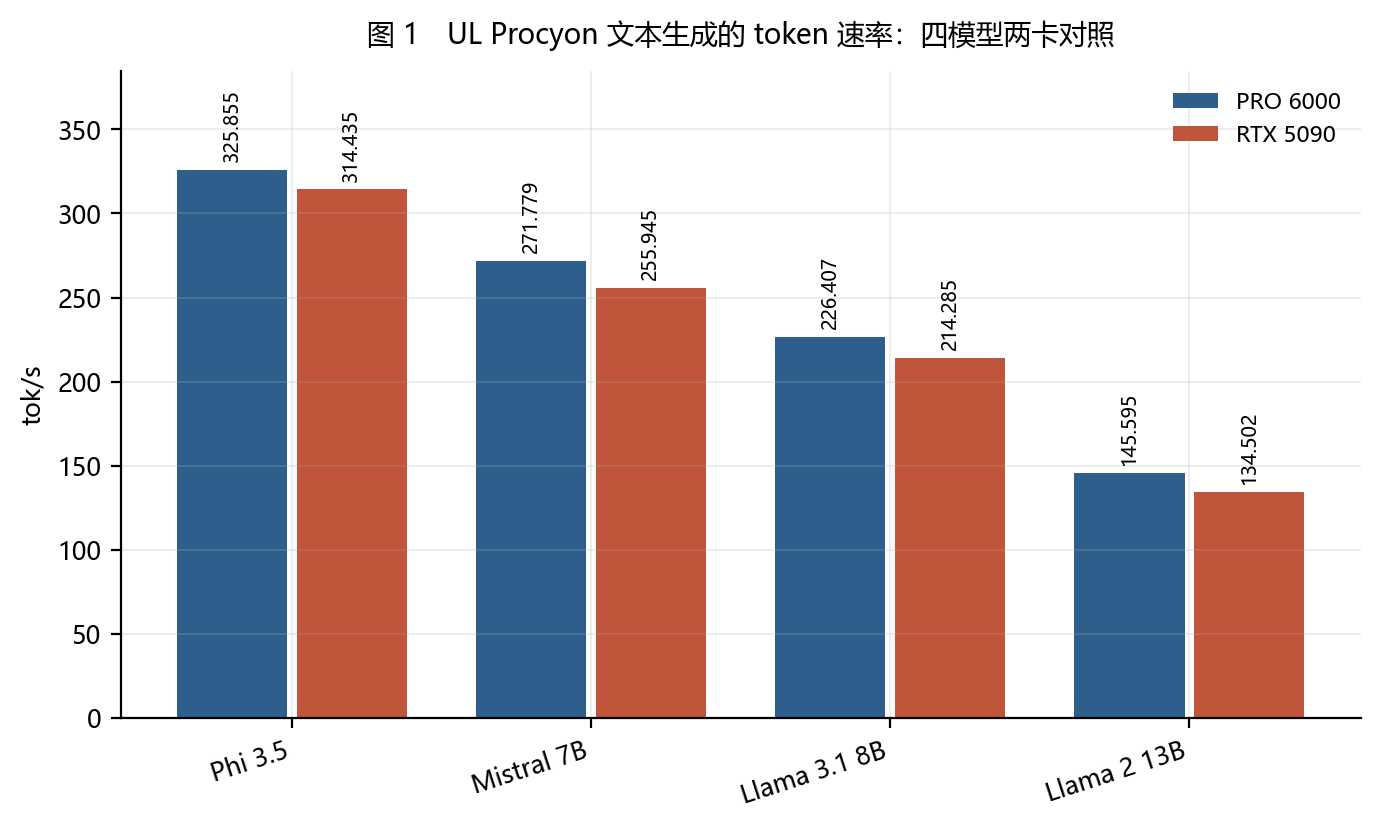
\includegraphics[width=0.86\textwidth]{../figures/fig-1.png}
\caption{图 1　UL Procyon 文本生成的 token 速率：四模型两卡对照。}
\label{fig:1}
\end{figure*}

图 1 把四个模型的 token 速率并排放在一起，可以看到 PRO 6000 的领先幅度随模型变小而收窄。


同一批评测、同一软件栈下（\texttt{WS} 版对 RTX 5090），四模型的 token 速率：


\begin{table*}[t]
\centering
\footnotesize
\setlength{\tabcolsep}{4pt}
\label{tab:5}
\begin{tabular}{llrl}
\toprule
模型 & WS 版 & RTX 5090 & WS 领先 \\
\midrule
Phi 3.5 & \textbf{325.855} & 314.435 & \textbf{3.6\%} \\
Mistral 7B & \textbf{271.779} & 255.945 & \textbf{6.2\%} \\
Llama 3.1 8B & \textbf{226.407} & 214.285 & \textbf{5.7\%} \\
Llama 2 13B & \textbf{145.595} & 134.502 & \textbf{8.2\%} \\
\bottomrule
\end{tabular}
\end{table*}

差距区间 \textbf{1.5\%-\hspace{0pt}5.9\%}（评测方口径），量级与噪声同阶 {\scriptsize\texttt{c-\hspace{0pt}sr-\hspace{0pt}token-\hspace{0pt}vs-\hspace{0pt}score}}。


\textbf{但同一测试的总分不是这个数。} Phi 总分 6,775 对 5,749（\textbf{+17.8\%}）、Mistral 7,346 对 6,267（\textbf{+17.2\%}）、Llama3 6,501 对 6,104（\textbf{+6.5\%}）、Llama2 8,008 对 6,591（\textbf{+21.5\%}）。


\begin{quote}\small
\textbf{\sym{⭐}{}\sym{⭐}{}\sym{⭐}{} 第一个方法论发现}

同一个基准同时输出「token 速率」和「综合总分」，两者幅度差 3 倍。原因是总分含首字延迟、加载时间与内存行为的加权，而 token 速率只测稳态解码。\textbf{故「Procyon 显示领先 18\%」与「Procyon 显示领先 5\%」都是真的，而它们说的是两件不同的事。}

\end{quote}

另一条独立佐证：INT8 量化推理上两者基本持平——79,064 对 79,272，\textbf{5090 反而高 0.3\%} {\scriptsize\texttt{c-\hspace{0pt}sr-\hspace{0pt}int8-\hspace{0pt}saturates}}。原作者的解释是 INT8 负载对显存带宽与容量的依赖较低。


\textbf{而 SKU 的影响在这里也被单独测到}：\texttt{MQ} 版对 RTX 5090 在低到中并发（1-\hspace{0pt}32）区间\textbf{稳定慢 11\%-\hspace{0pt}13\%}，原因是 575 W 对 300 W 的功耗预算差异，而非核心数 {\scriptsize\texttt{c-\hspace{0pt}j8-\hspace{0pt}maxq-\hspace{0pt}vs-\hspace{0pt}5090}}。


\begin{quote}\small
\textbf{\sym{⭐}{}\sym{⭐}{}\sym{⭐}{} 把这两条放在一起，得到一个反直觉的结论}

同一个「RTX PRO 6000」：\textbf{600 W 的 \texttt{WS} 版比 5090 快 5\%；300 W 的 \texttt{MQ} 版比 5090 慢 12\%。}故「这张卡比 5090 快还是慢」的答案，\textbf{取决于你买的是哪个 SKU}，而不取决于你测的是什么模型。

\end{quote}


\subsection{四档证据的对照}

表 1 把本文四组关键数据的场景、数值与证据等级并列。\textbf{这是全文唯一一张把「数字」与「它能证明什么」放在同一行的表。}


<!-- tables/tab-1.md -->

\begin{table*}[t]
\centering
\footnotesize
\setlength{\tabcolsep}{4pt}
\caption{四个推理档位的对照（含证据等级）。}
\label{tab:6}
\begin{tabularx}{\textwidth}{llrllX}
\toprule
档位 & 场景 & 关键数值 & 单位 & 证据等级 & 为何是这一级 \\
\midrule
容量不受约束 & Mistral 7B 解码 & 271.779 & tok/s & 测量级 & 同批评测同软件栈，但只有单一实验室 \\
容量不受约束 & INT8 量化推理 & 79064 & score & 测量级 & 对位 5090 为 79272，差距 0.3\% 在噪声内 \\
容量成为约束 & GPT-OSS 120B & 163.15 & tok/s & 测量级 & 5090 无法加载该模型，故这是单选题而非对比 \\
容量成为约束 & Llama 3.3 70B 对 5090 & 928 & 百分比 & 诊断级 & 提升来自对方显存耗尽而非算力差 \\
\bottomrule
\end{tabularx}
\end{table*}


\subsection{往上比：与 H100 / B200 / GB300 的对位}

前一小节比的是消费级（5090、4090、6000 Ada）。真正决定这张卡定位的是往上一档：它到底能不能替代 H100？本节的答案是\textbf{分维度}的，而每一维的答案都不同。


\subsubsection{规格层：一赢一平三输}

SLAC 给出了一份逐项规格对比，并注明「来自数据表而非在自家内核上实测」{\scriptsize\texttt{c-\hspace{0pt}slac-\hspace{0pt}h100-\hspace{0pt}vs-\hspace{0pt}rtx}}：


\begin{table*}[t]
\centering
\footnotesize
\setlength{\tabcolsep}{4pt}
\label{tab:7}
\begin{tabular}{llll}
\toprule
维度 & RTX PRO 6000 & H100 NVL & 领先方 \\
\midrule
FP32 & 约 125 TFLOPS & 约 60 TFLOPS & \textbf{RTX 领先 2.1 倍} \\
FP64 & 约 2.0 TFLOPS & 约 30 TFLOPS & H100 领先 15 倍 \\
显存带宽 & 1.79 TB/s & 3.9 TB/s & H100 领先 2.2 倍 \\
价格（2026-07） & 约 \$13,000 & 约 \$28,000 & \textbf{RTX 便宜 2.1 倍} \\
\bottomrule
\end{tabular}
\end{table*}

\textbf{FP32 赢 2.1 倍、价格赢 2.1 倍，而 FP64 输 15 倍、带宽输 2.2 倍。}


\begin{figure*}[t]
\centering
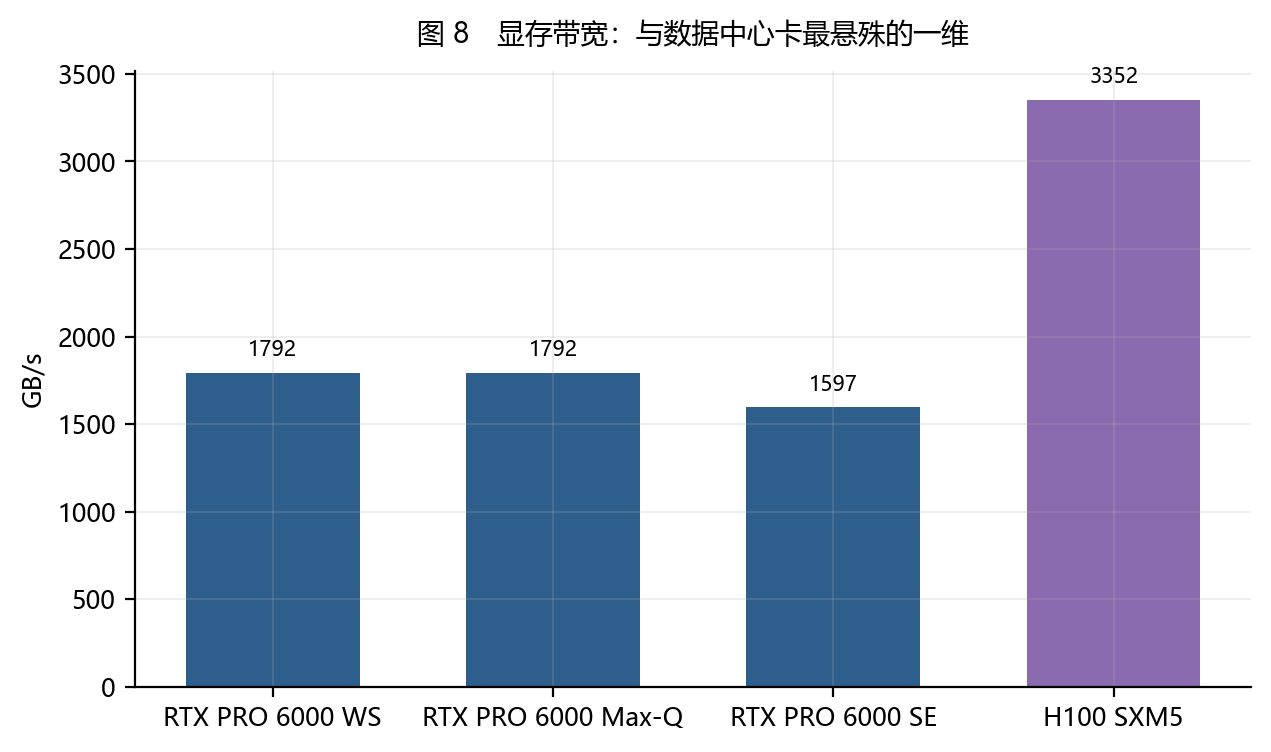
\includegraphics[width=0.86\textwidth]{../figures/fig-8.png}
\caption{图 8　显存带宽：与数据中心卡最悬殊的一维。}
\label{fig:2}
\end{figure*}

图 8 只画了四个有确切数值的档位，把这张卡与数据中心卡的差距压缩成一个可以一眼比较的高度差。


带宽是本节最关键的一维，因为\textbf{解码是带宽受限的}：H100 SXM5 的 3,352 GB/s 是这张卡 1,792 GB/s 的 \textbf{1.87 倍} {\scriptsize\texttt{c-\hspace{0pt}hbm-\hspace{0pt}bw-\hspace{0pt}gap}}，GH200 约 4.0 TB/s（\textbf{2.2 倍}）。而 H100 NVL 在 SLAC 的对照里记为「约 3.9 TB/s」{\scriptsize\texttt{c-\hspace{0pt}slac-\hspace{0pt}h100-\hspace{0pt}vs-\hspace{0pt}rtx}}。图 8 只画了有确切数值的四档；后两个在来源里是「约」值，故不画柱以避免伪造精度。


\begin{quote}\small
\textbf{\sym{⭐}{}\sym{⭐}{}\sym{⭐}{} 判据}

故在\textbf{单流解码}这个最常被引用的场景里，这张卡在物理上不可能追上 H100：因为解码每生成一个 token 都要读一遍权重，而读的速度差 1.87 倍。

\textbf{而它在 FP32 上赢的 2.1 倍，对这个场景完全无用。}

这就是「跑分赢、推理输」的物理原因，不是软件问题。

\end{quote}

\subsubsection{互连层：PCIe 对 NVLink，差 66\%}

\begin{figure*}[t]
\centering
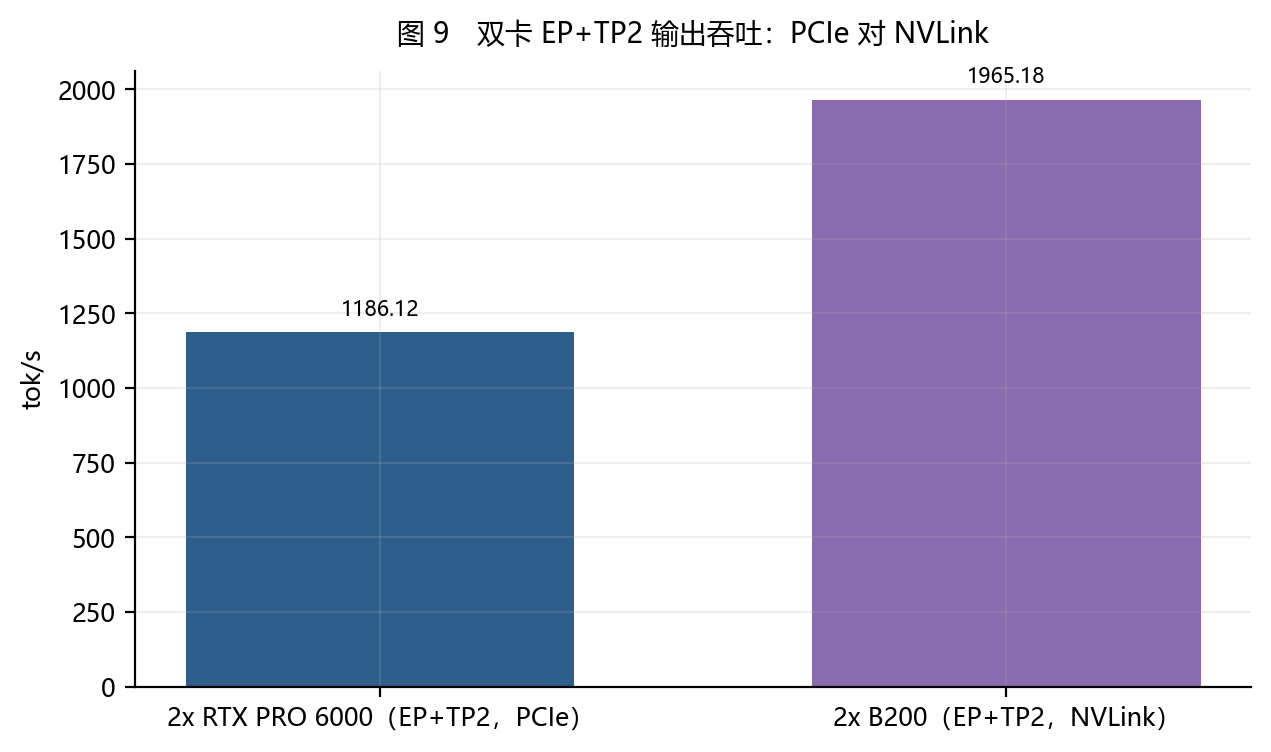
\includegraphics[width=0.86\textwidth]{../figures/fig-9.png}
\caption{图 9　双卡 EP+TP2 输出吞吐：PCIe 对 NVLink。}
\label{fig:3}
\end{figure*}

图 9 的两组柱子共用同一套并行配置，故 66\% 的差距只能归因于互连。


一条对照组数据把互连的代价单独量了出来 {\scriptsize\texttt{c-\hspace{0pt}ep-\hspace{0pt}gap}}：同为双卡、\textbf{同开 EP+TP2}，2× B200（NVLink）输出 \textbf{1,965 tok/s}，2× RTX PRO 6000（PCIe）为 \textbf{1,186 tok/s}；TPOT \textbf{5.63 ms 对 12.82 ms}（快 2.3 倍）。


\begin{quote}\small
\textbf{\sym{⭐}{}\sym{⭐}{} 判据}

这是本文唯一一条「只换互连、不换算力」的对照，故它测的是 \textbf{PCIe 与 NVLink 的差，不是两张卡的差}。

而它给出的量级（66\% 吞吐、2.3 倍 TPOT）意味着：任何多卡推理的对比，只要一侧有 NVLink 另一侧没有，\textbf{这个差就会混进「卡间性能差」里而无法分离}：除非像这条一样把 EP+TP2 固定住。

\end{quote}

\subsubsection{成本层：买得起不等于用得起}

这是三种相反结论里最尖锐的一种：\textbf{按芯片成本排它最低，按 token 成本排它最高。}


具体数字、并发差异与全部八个指标见 \textbf{§9}——那一章专门处理成本，因为这里若展开，就会与那里重复同一组数。


\begin{quote}\small
\textbf{\sym{⭐}{}\sym{⭐}{}\sym{⭐}{} 判据}

\textbf{成本比的分子必须是「每单位产出」，而不是「每单位时间」。}这不是定价策略的差别，是\textbf{分母选错}的差别。

\end{quote}

\subsubsection{功耗层：两个指标指向不同的卡}

还有一维必须单列，因为它与前几维的结论相反 {\scriptsize\texttt{c-\hspace{0pt}slac-\hspace{0pt}power-\hspace{0pt}favors-\hspace{0pt}h100}}：在机架密度下，H100 约领先 \textbf{1.5 倍性能每瓦}。


\begin{quote}\small
\textbf{\sym{⭐}{}\sym{⭐}{} 判据}

至此这张卡的定位在三个指标上是\textbf{三种结论}：\textbf{每美元性能}赢（便宜 2.1 倍）、\textbf{每瓦性能}输（落后 1.5 倍）、\textbf{每 token 成本}大输（差 9.5 倍）。

故「RTX PRO 6000 与 H100 谁更好」这个问题\textbf{没有单一答案}，只有「在哪个约束下更好」。

\end{quote}


\subsection{往下比：与上代专业卡的对照}

比消费级是「值不值」，比数据中心是「能不能替代」，而比上代是\textbf{升级决策}里最实际的一问：我这台机器上的 RTX 6000 Ada 或 L40S，换不换？


本节的答案是：\textbf{同一张卡对上代有六个倍率，从 1.09 到 21.3，而它们都不假。}


\begin{table*}[t]
\centering
\footnotesize
\setlength{\tabcolsep}{4pt}
\caption{与上代专业卡的对照（按口径分行）。}
\label{tab:8}
\begin{tabular}{llllrl}
\toprule
对照对象 & 维度 & 上代数值 & 本代数值 & 倍率 & 口径 \\
\midrule
RTX 6000 Ada & 显存容量 & 48 GB & 96 GB & 2.0 & 规格 \\
RTX 6000 Ada & 显存带宽 & 960 GB/s & 1792 GB/s & 1.87 & 规格 \\
RTX 6000 Ada & L2 缓存 & 98304 KB & 131072 KB & 1.33 & 规格 \\
RTX A6000 & L2 缓存 & 6144 KB & 131072 KB & 21.3 & 规格 \\
RTX 6000 Ada & SPECviewperf 15 几何均值 & 1.0 & 1.47 & 1.47 & 实测渲染 \\
RTX 6000 Ada & SPECviewperf 15 中位数 & 1.0 & 1.31 & 1.31 & 实测渲染 \\
L40 Ada & 多基准中位吞吐 & 1.0 & 1.09 & 1.09 & 实测推理 \\
L40 Ada & 多基准吞吐 p90 & 1.0 & 1.28 & 1.28 & 实测推理 \\
L40 Ada & 厂商宣称 Llama 3 70B 加速 & 1.0 & 5.6 & 5.6 & 厂商声明 \\
L40S & Parabricks Fastq2bam & 1.0 & 1.5 & 1.5 & 厂商声明 \\
\bottomrule
\end{tabular}
\end{table*}

\subsubsection{规格倍率最容易骗人}

先看两个最悬殊的规格项。容量从 48 GB 到 96 GB（\textbf{2.0 倍}）、带宽从 960 GB/s 到 1,792 GB/s（\textbf{1.87 倍}）{\scriptsize\texttt{c-\hspace{0pt}gen-\hspace{0pt}gain}}。


而 L2 缓存从 RTX 6000 Ada 的 98,304 KB 到 131,072 KB（\textbf{1.33 倍}），若与更早的 RTX A6000 的 6,144 KB 相比则是 \textbf{21.3 倍} {\scriptsize\texttt{c-\hspace{0pt}l2-\hspace{0pt}cache}}。


\begin{quote}\small
\textbf{\sym{⭐}{}\sym{⭐}{}\sym{⭐}{} 判据}

\textbf{21.3 倍这个数字是真的，但它对推理性能的意义接近于零。}因为 L2 缓存的收益取决于工作集能否装进去，而不取决于「比三代前大多少倍」。

故\textbf{同一个「代际提升」，选不同的基线可以差 20 倍。}说「提升 N 倍」而不说「相对谁」，等于没有信息。

\end{quote}

\subsubsection{实测：显存差 2 倍，吞吐只差 1.09 倍}

\begin{figure*}[t]
\centering
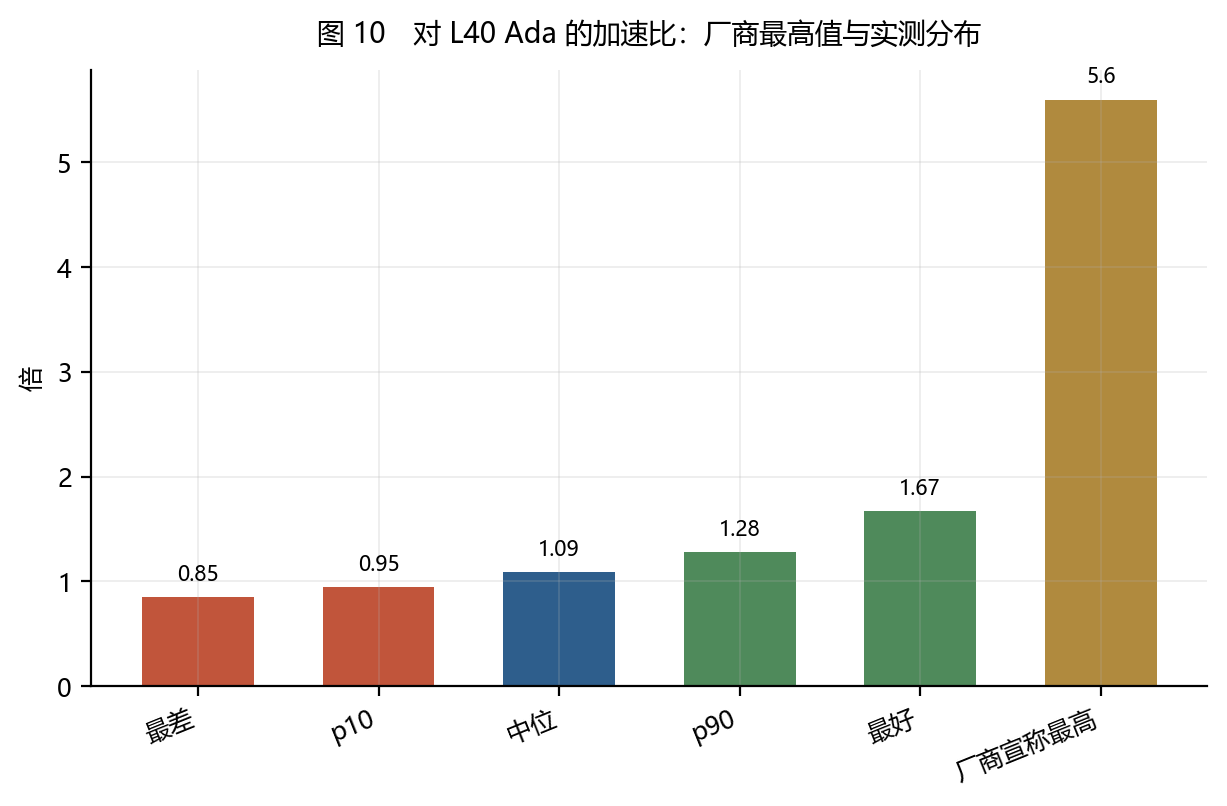
\includegraphics[width=0.86\textwidth]{../figures/fig-10.png}
\caption{图 10　对 L40 Ada 的加速比：厂商最高值与实测分布。}
\label{fig:4}
\end{figure*}

图 10 把六个倍率画在同一条数轴上，从 0.85 到 5.6 的跨度就是本节的全部论点。


一份多基准实测给出了完整的分布 {\scriptsize\texttt{c-\hspace{0pt}omni3-\hspace{0pt}vs-\hspace{0pt}l40-\hspace{0pt}median}}：相对 L40 Ada，\textbf{中位加速比 1.09 倍、胜率 78\%}，p10 为 0.95、p90 为 1.28、最差 0.85 倍、最好 1.67 倍。


\textbf{即两卡显存差 2.0 倍，而实际吞吐差中位仅 1.09 倍。}


而厂商的宣传口径是\textbf{最高 5.6 倍}（Llama 3 70B）{\scriptsize\texttt{c-\hspace{0pt}vgpu-\hspace{0pt}l40s-\hspace{0pt}56}}，分项为 Siemens UFX 2.3 倍、Dassault Abaqus 2 倍、Autodesk Arnold 1.9 倍、Omniverse 3.5 倍。


\begin{quote}\small
\textbf{\sym{⭐}{}\sym{⭐}{}\sym{⭐}{}\sym{⭐}{}\sym{⭐}{} 判据}

\textbf{0.85 倍与 5.6 倍是同一对显卡。}

前者是实测分布的最差值，后者是厂商选的单点最优。两者都不假，但\textbf{并列才看得出「最高值」离典型值有多远}——中位 1.09 倍意味着：\textbf{换卡的一半场景里，你几乎感觉不到差别。}

故采购判据不能是「最高加速比」，必须是\textbf{你自己负载上的中位数}。

\end{quote}

而 p10 为 0.95 倍这个数值得单独说：\textbf{有 10\% 的基准上，新卡比上代还慢。}


\subsubsection{渲染：这一代是实打实的}

并非所有维度都这么平。SPECviewperf 15 上（同为 4K），相对 RTX 6000 Ada 的\textbf{几何平均提升 1.47 倍、中位数 1.31 倍} {\scriptsize\texttt{c-\hspace{0pt}vp15-\hspace{0pt}vs-\hspace{0pt}ada}}。


而各项差异极大：enscape-01 达 \textbf{2.40 倍}、blender-01 \textbf{2.10 倍}，而 unreal\_engine-01 仅 \textbf{1.11 倍}。


\begin{quote}\small
\textbf{\sym{⭐}{}\sym{⭐}{} 判据}

渲染的中位 1.31 倍高于推理的中位 1.09 倍。原因不神秘：\textbf{渲染是算力受限，推理是带宽受限}。这一代算力涨得多、带宽涨得少（1.87 倍），故两类负载的收益不同。

这与 §3.2 的结论同源：\textbf{带宽是这张卡的短板，而它恰好是推理的瓶颈。}

\end{quote}

\subsubsection{一条反例：Parabricks 上代际与档位同时被跨越}

Parabricks 的 Fastq2bam+DeepVariant 上，Server Edition 比 L40S 快 \textbf{1.5 倍}、比 H100 快 \textbf{1.75 倍} {\scriptsize\texttt{c-\hspace{0pt}parabricks}}。


\begin{quote}\small
\textbf{\sym{⭐}{}\sym{⭐}{} 判据}

这是本文少见的一条「跨代 + 跨档都赢」的负载。它的存在说明：\textbf{上述所有倍率都是「在该负载上」的，没有一条是「这张卡」的属性。}

\end{quote}


\subsection{预填与解码是两条曲线，不是一条}

前面三节都在回答「这张卡多快」。本节要说的是：\textbf{这个问题本身有歧义。}


\begin{figure*}[t]
\centering
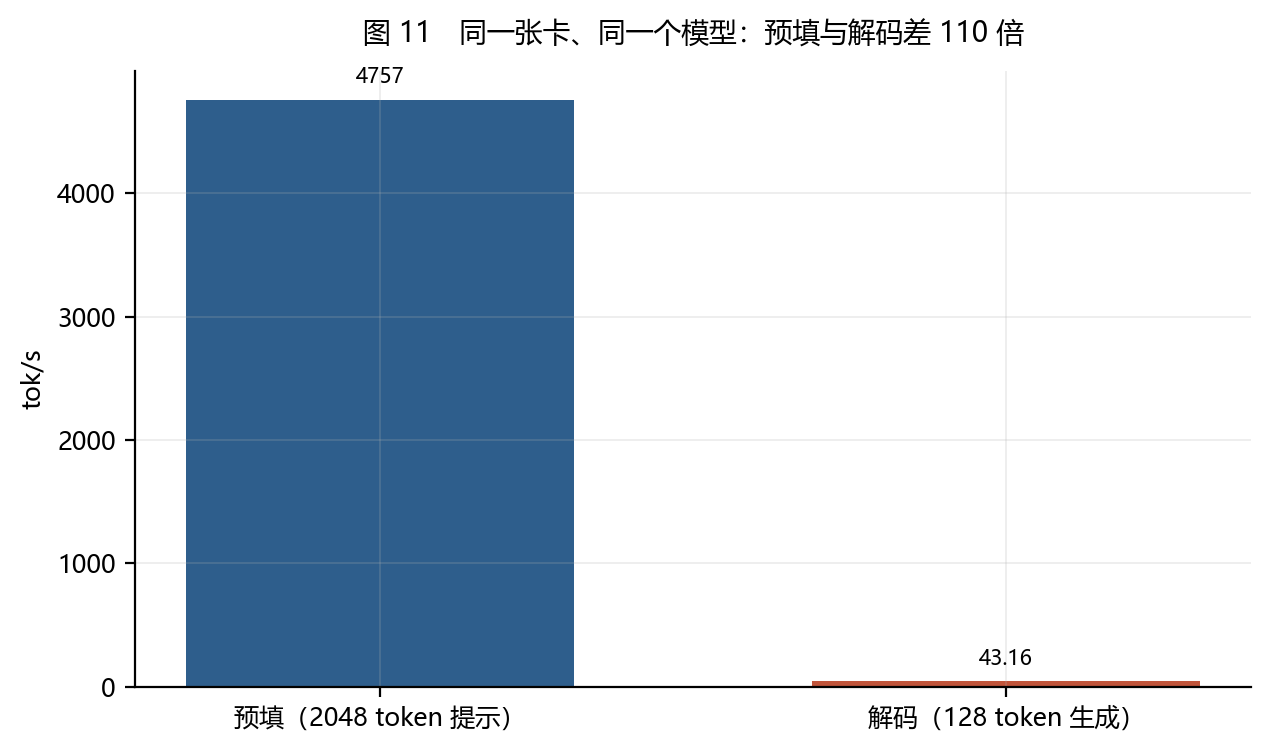
\includegraphics[width=0.86\textwidth]{../figures/fig-11.png}
\caption{图 11　同一张卡、同一个模型：预填与解码差 110 倍。}
\label{fig:5}
\end{figure*}

图 11 的两根柱子来自\textbf{同一套 llama.cpp 单流测量、同一张 RTX PRO 6000}：Qwen3.8-27B-Q8\_0 的预填 \textbf{4,757 tok/s}，解码 \textbf{43.16 tok/s} {\scriptsize\texttt{c-\hspace{0pt}llamacpp-\hspace{0pt}prefill}}{\scriptsize\texttt{c-\hspace{0pt}llamacpp-\hspace{0pt}decode-\hspace{0pt}parity}}。


\textbf{相差 110 倍。} 没有任何一对显卡之间的差距有这个量级。


\begin{table*}[t]
\centering
\footnotesize
\setlength{\tabcolsep}{4pt}
\caption{预填与解码：两条完全不同的性能曲线。}
\label{tab:9}
\begin{tabularx}{\textwidth}{llX}
\toprule
维度 & 预填（prefill） & 解码（decode） \\
\midrule
处理对象 & 整段提示 可并行 & 逐 token 生成 串行 \\
瓶颈 & 算力 FLOPS & 显存带宽 GB/s \\
实测量级（同卡同模型） & 4757 tok/s & 43.16 tok/s \\
受功耗档位影响 & 明显 WS 比 MQ 约快 20\% & 很小 原文作 similar \\
同为 1792 GB/s 的两卡 & 可以差出数倍 & 接近持平 near-parity \\
受互连影响 & 中等 & 高 EP+TP2 上 PCIe 对 NVLink 差 66\% \\
长输入的代价 & 随输入长度线性增长 & 不变 \\
长输出的代价 & 不变 & 累积下降 可至 6-9 tok/s \\
谁更快的答案取决于 & 算力与功耗档位 & 带宽与互连 \\
\bottomrule
\end{tabularx}
\end{table*}

\subsubsection{机制：一个并行，一个串行}

预填处理整段提示，所有 token 可以同时算——\textbf{瓶颈是算力}。解码逐 token 生成，每一步都要把整个模型的权重从显存读一遍——\textbf{瓶颈是带宽}。


\begin{quote}\small
\textbf{\sym{⭐}{}\sym{⭐}{}\sym{⭐}{}\sym{⭐}{}\sym{⭐}{} 判据}

\textbf{这两件事对硬件的要求几乎正交，故它们对同一张卡的排序也不同。}

一个只看预填的评测与一个只看解码的评测，可以给出相反的采购建议，而两者都没有说谎。

\end{quote}

\subsubsection{三条互相印证的证据}

\textbf{其一，同带宽的两张卡，解码持平。}PRO 6000 与 RTX 5090 都标 1,792 GB/s，在 llama.cpp 单流解码下接近持平——来源自己的说法是「near-parity is the reasonable batch-one decode hypothesis」{\scriptsize\texttt{c-\hspace{0pt}llamacpp-\hspace{0pt}decode-\hspace{0pt}parity}}。


\textbf{其二，功耗档位只影响预填。}Max-Q（300 W）与 Workstation（600 W）相比，原文是「\textasciitilde{}20\% faster prefill on WS, similar decode speed (VRAM/PCIe limited)」{\scriptsize\texttt{c-\hspace{0pt}6kw-\hspace{0pt}maxq-\hspace{0pt}prefill}}。


即\textbf{多给一倍功耗，预填快两成，解码几乎不动}——因为解码本来就不受算力限制。


\textbf{其三，互连只在解码上分出高下。}双卡 EP+TP2 上，2 张 PRO 6000（PCIe）对 2 张 B200（NVLink）：输出吞吐 1,186 对 1,965 tok/s、TPOT 12.82 对 5.63 ms {\scriptsize\texttt{c-\hspace{0pt}ep-\hspace{0pt}gap}}。\textbf{多卡解码要每步同步，故互连延迟直接进入关键路径。}


\subsubsection{代价的形状也不同}

「长上下文慢」这个说法同样要拆开。输入变长只推高预填成本（线性增长），输出变长才压解码吞吐；而长输出下的解码会累积下降到 \textbf{6-\hspace{0pt}9 tok/s} {\scriptsize\texttt{c-\hspace{0pt}long-\hspace{0pt}sustained-\hspace{0pt}gen-\hspace{0pt}degrades}}。


\begin{quote}\small
\textbf{\sym{⭐}{}\sym{⭐}{}\sym{⭐}{} 判据}

故 §5.4 那张图的两条曲线为什么形状不同，这里给出了原因：\textbf{一条是输入变长，一条是输出变长，它们加压在不同的瓶颈上。}

\end{quote}

\subsubsection{对选型的直接含义}

如果你的负载是\textbf{长提示、短回答}（检索增强、文档问答、代码补全），那么这张卡的短板（带宽）基本不出现，它是一张很快的卡。


如果是\textbf{短提示、长回答}（自由生成、思维链、agent 循环），那么几乎全部时间花在解码上，而解码恰好是它相对数据中心卡最弱的一维。


\begin{quote}\small
\textbf{\sym{⭐}{}\sym{⭐}{}\sym{⭐}{}\sym{⭐}{} 判据}

\textbf{同一张卡可以是「性价比极高」也可以是「明显不够」，取决于回答有多长。}

这就是为什么本文从头到尾拒绝给一个单一的「快多少倍」。

\end{quote}


\subsection{首字延迟是第三个维度，和上面两个都不同步}

§3.4 把「多快」拆成预填与解码两半。这一节再拆出一维：\textbf{第一个字要等多久}，即首字延迟（TTFT，time to first token）。


\begin{figure*}[t]
\centering
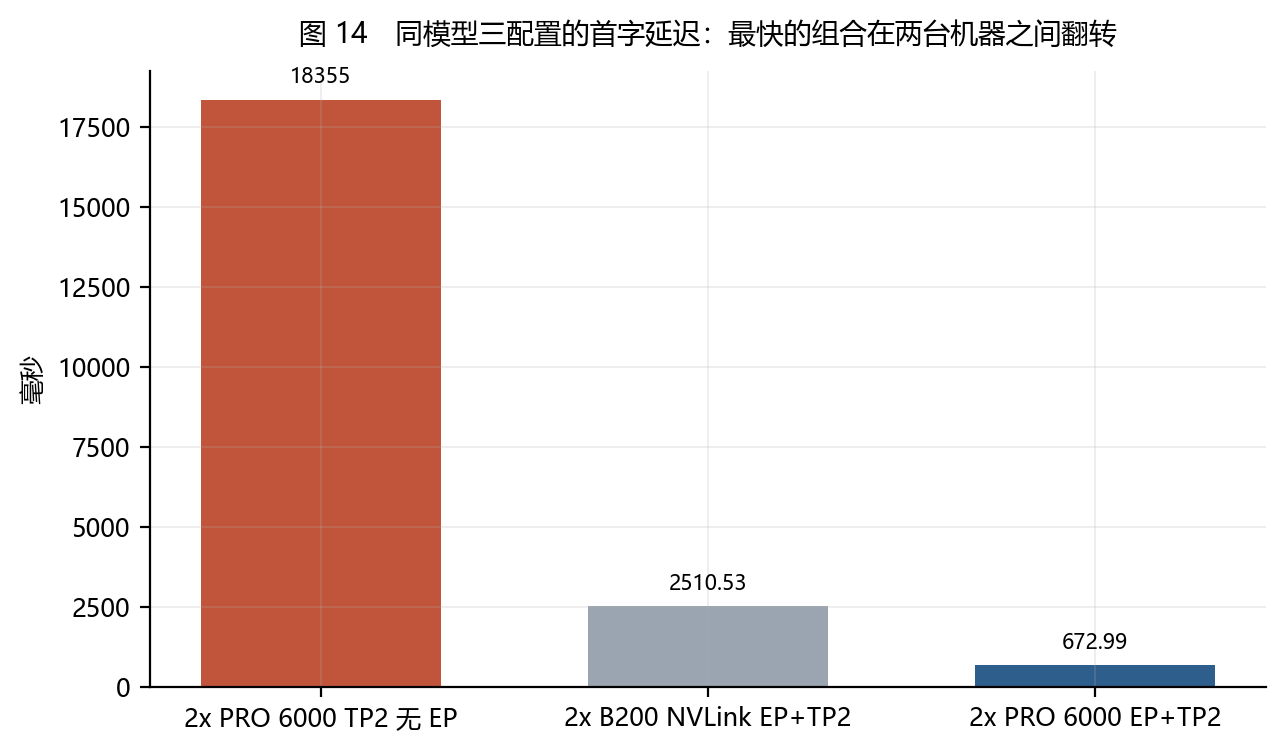
\includegraphics[width=0.86\textwidth]{../figures/fig-14.png}
\caption{图 14　同模型三配置的首字延迟：最快的组合在两台机器之间翻转。}
\label{fig:6}
\end{figure*}

图 14 的三根柱子是同一个模型（Qwen3.5-35B-A3B）、两种互连下的三种配置。注意纵轴\textbf{越低越好}，且最高的那根比最低的高 \textbf{27 倍}。


\begin{table*}[t]
\centering
\footnotesize
\setlength{\tabcolsep}{4pt}
\caption{首字延迟、吞吐与 TPOT 三者不同步。}
\label{tab:10}
\begin{tabular}{lrrrl}
\toprule
配置 & TTFT 毫秒 & 输出吞吐 tok/s & TPOT 毫秒 & 互连 \\
\midrule
2x PRO 6000 TP2 无 EP & 18354.95 & 516.44 & 12.63 & PCIe \\
2x PRO 6000 EP+TP2 & 672.99 & 1186.12 & 12.82 & PCIe \\
2x B200 NVLink EP+TP2 & 2510.53 & 1965.18 & 5.63 & NVLink \\
\bottomrule
\end{tabular}
\end{table*}

\subsubsection{三列给出三种排序}

表 9 最值得看的地方不是数字，而是\textbf{三列排出的三种名次}：


\begin{itemize}
  \item 按\textbf{首字延迟}：2x PRO 6000 开 EP（673 ms）快于 2x B200（2,511 ms），快 3.7 倍
  \item 按\textbf{输出吞吐}：2x B200（1,965 tok/s）快于 2x PRO 6000 开 EP（1,186），快 1.66 倍
  \item 按\textbf{TPOT}：2x B200（5.63 ms）快于 2x PRO 6000（12.82 ms），快 2.3 倍
\end{itemize}

\begin{quote}\small
\textbf{\sym{⭐}{}\sym{⭐}{}\sym{⭐}{}\sym{⭐}{}\sym{⭐}{} 判据（本文第三条）}

\textbf{首字延迟由「要等多久才开始算」决定，解码吞吐由「算起来多快」决定，而这两件事在多卡上由不同的东西支配。}

前者受\textbf{同步次数}影响：EP 把整个 MoE 层的激活不再全卡同步，于是 18,355 ms 变成 673 ms；后者受\textbf{互连带宽}影响：B200 的 NVLink 让每步同步更快。

\end{quote}

\subsubsection{的收益几乎全在首字上}

同一对 PRO 6000、同一模型，开 EP 前后 {\scriptsize\texttt{c-\hspace{0pt}ep-\hspace{0pt}ttft}}：


\begin{table*}[t]
\centering
\footnotesize
\setlength{\tabcolsep}{4pt}
\label{tab:11}
\begin{tabular}{llll}
\toprule
 & 无 EP & EP+TP2 & 变化 \\
\midrule
首字延迟 & 18,355 ms & \textbf{673 ms} & \textbf{快 27 倍} \\
输出吞吐 & 516 tok/s & 1,186 tok/s & 快 2.3 倍 \\
TPOT & 12.63 ms & 12.82 ms & \textbf{几乎不变} \\
\bottomrule
\end{tabular}
\end{table*}

\textbf{TPOT 基本没动。} 这说明 EP 改善的不是「每个字出得多快」，而是「开始出第一个字之前的那段等待」。


\begin{quote}\small
\textbf{\sym{⭐}{}\sym{⭐}{}\sym{⭐}{} 判据}

故「开了 EP 快 27 倍」这句话\textbf{只对首字成立}。若用它去描述吞吐，会夸大 12 倍；若用它描述 TPOT，会夸大无穷倍。

\end{quote}

\subsubsection{而 B200 在首字上反而更慢}

同一份基准里，2x B200 靠 NVLink 拿到更高的吞吐与更低的 TPOT，但首字延迟是 \textbf{2,511 ms}，比 2x PRO 6000 开 EP 的 673 ms 慢 3.7 倍 {\scriptsize\texttt{c-\hspace{0pt}ep-\hspace{0pt}gap}}。


\sym{⭐}{} 这不是 B200 弱，而是\textbf{两台机器的瓶颈位置不同}：B200 的优势在卡间带宽（每步同步更快），PRO 6000 的优势在单卡容量（同样的模型可以用更少的卡装下，于是同步更少）。


\begin{quote}\small
\textbf{\sym{⭐}{}\sym{⭐}{}\sym{⭐}{}\sym{⭐}{} 判据}

\textbf{首字延迟与吞吐可以为不同的卡各自最优，且差距都在数倍量级。}

故一个只报吞吐的评测与一个只报首字的评测，会给出相反的采购建议，而两者都没有说谎——这与 §3.4 的结论是同一件事的第二次出现。

\end{quote}

\subsubsection{单卡部署的天然优势}

单卡没有跨卡通信，故 8B 模型的首字延迟是 \textbf{205 ms}，而多卡或跨节点方案在同一档位上是 \textbf{520 到 1,320 ms} {\scriptsize\texttt{c-\hspace{0pt}ttft-\hspace{0pt}advantage}}。


\sym{⭐}{} 这是 96 GB 的另一个收益，而它与容量无关：\textbf{能装下就不必分卡，不必分卡就没有首字前的同步等待。}


而 MTP（多 token 预测）这类加速技术的收益分布也印证了同一条线：并发 1 时 P95 首字延迟只从 198 ms 降到 179 ms，\textbf{收益集中在解码阶段而非预填阶段} {\scriptsize\texttt{c-\hspace{0pt}mtp-\hspace{0pt}ttft-\hspace{0pt}barely}}。



\section{容量成为约束时的推理性能}

这一节的所有数字都属于\textbf{另一类比较}：不是「谁在同任务上更快」，而是「谁能跑」。


\begin{figure*}[t]
\centering
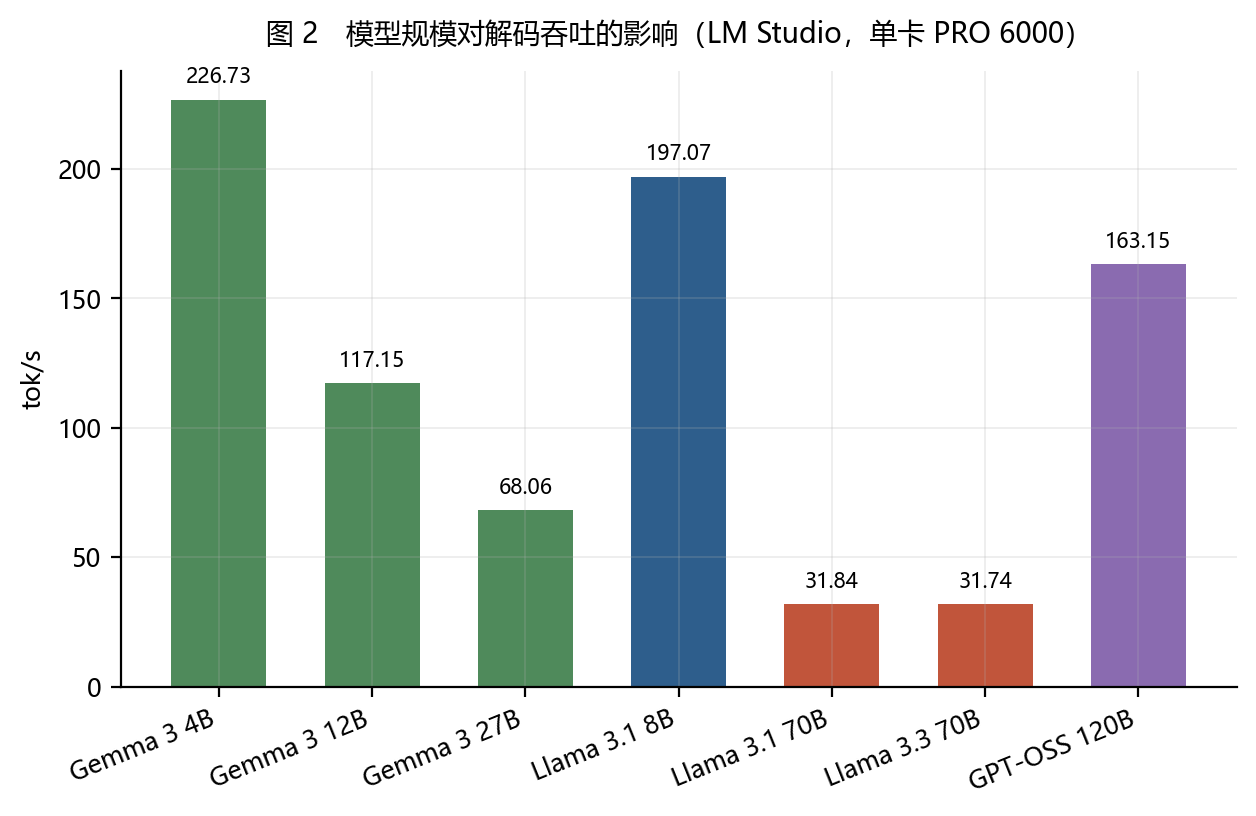
\includegraphics[width=0.86\textwidth]{../figures/fig-2.png}
\caption{图 2　模型规模对解码吞吐的影响（LM Studio，单卡，SKU 未指明）。}
\label{fig:7}
\end{figure*}

图 2 的横轴是模型规模，纵轴是解码吞吐，两条曲线的间距随规模增大而拉开。


同一 500 词提示、Q4 量化：


\begin{table*}[t]
\centering
\footnotesize
\setlength{\tabcolsep}{4pt}
\label{tab:12}
\begin{tabular}{llll}
\toprule
模型 & 规模 & tok/s & 备注 \\
\midrule
Gemma 3 4B & 4B & \textbf{226.73} &  \\
Llama 3.1 8B & 8B & 197.07 &  \\
Gemma 3 12B & 12B & 117.15 &  \\
Gemma 3 27B & 27B & 68.06 &  \\
Llama 3.1 70B & 70B & 31.84 & Q4\_K\_S \\
Llama 3.3 70B & 70B & 31.74 & Q4\_K\_S \\
\textbf{GPT-OSS 120B} & 120B MoE & \textbf{163.15} & 首字 0.193 s \\
\bottomrule
\end{tabular}
\end{table*}

\textbf{\sym{⚠}{} 这一组数据来源只写「RTX PRO 6000」，未指明 SKU。} 按其 120B 的 163.15 tok/s 与同系列 \texttt{MQ} 的 120B 数据（170.62）接近，推测为 \texttt{MQ} 或 \texttt{WS}，但在来源明确前不应断言。


两种读法都成立，而它们是不同的结论：


\begin{enumerate}
  \item \textbf{纵向}：4B \sym{→}{} 70B 吞吐降了 \textbf{7 倍}，密模型规模与吞吐近似反比。
  \item \textbf{横向}：120B 的 MoE 反而比 70B 密模型快 \textbf{5 倍}。
\end{enumerate}

\begin{quote}\small
\textbf{\sym{⭐}{}\sym{⭐}{}\sym{⭐}{} 故「参数量」不是吞吐的单调预测因子。}真正决定解码速度的是\textbf{每 token 需要搬运的活跃字节数}，而 MoE 把「总参数」与「活跃参数」解耦了。

\end{quote}

\textbf{而这一节真正的分界线在这里：RTX 5090 无法加载 120B 模型，甚至常处理不了 70B} {\scriptsize\texttt{c-\hspace{0pt}sr-\hspace{0pt}96gb-\hspace{0pt}unique}}。


Llama 3.3 70B Q4\_K\_S 上，比 5090 提升 \textbf{928\%}、比 4090 提升 \textbf{1141\%} {\scriptsize\texttt{c-\hspace{0pt}gn-\hspace{0pt}70b-\hspace{0pt}capacity-\hspace{0pt}domain}}。


\begin{quote}\small
\textbf{\sym{⚠}{}\sym{⚠}{}\sym{⚠}{} 这三个百分比的正确读法}

它们的量级差距不来自算力，而来自\textbf{显存容量}：到某个点，其它卡显存耗尽，于是「比较」变成了「单边可用」。\textbf{故它不是一条性能结论，而是一条容量结论。}

\end{quote}


\section{DeepSeek-V4 / V4.1-Flash：本报告实测最多的一条模型线}

前四节讨论的是「这张卡」，本节讨论「这个模型」。这样做是因为DeepSeek-V4/4.1-Flash 在档案里有 \textbf{50 条主张、跨 6 种硬件配置}，是唯一一条能在同一张卡上横向看到「预填 / 解码 / 长上下文 / 投机解码」四个维度的模型线。


\subsection{先给结论：一个模型，三个数量级}

把档案里所有 DeepSeek-V4-Flash 的数字放在一起，会得到一个看起来荒谬的结果：


\begin{table*}[t]
\centering
\footnotesize
\setlength{\tabcolsep}{4pt}
\label{tab:13}
\begin{tabular}{lll}
\toprule
场景 & 硬件 & 数值 \\
\midrule
单流解码（原生 FP8 热态） & 2× DGX Spark TP2 & \textbf{44 tok/s} \\
单流解码（Q8 无投机） & 2× PRO 6000 & \textbf{46 tok/s} \\
单流解码（300 W 目录值） & 1× PRO 6000 @300W & \textbf{102.7 tok/s} \\
解码（同批预填测试） & 2× PRO 6000 WS TP2 & \textbf{133.7 tok/s} \\
预填 8k（混合方案） & 2× PRO 6000 WS TP2 & \textbf{13,811 tok/s} \\
预填 128k（混合方案） & 2× PRO 6000 WS TP2 & \textbf{12,182 tok/s} \\
\bottomrule
\end{tabular}
\end{table*}

从 44 到 13,811，跨 \textbf{三个数量级}。而它们都是真的。


\begin{quote}\small
\textbf{\sym{⭐}{}\sym{⭐}{}\sym{⭐}{} 判据}

这不是数据矛盾，而是\textbf{测法不同}：预填（prefill）处理的是整段提示，可并行；解码（decode）逐 token 生成，受显存带宽约束。两者在同一个模型上天然差 100 倍以上。

\textbf{故「DeepSeek-V4-Flash 的吞吐是多少」这个问题，必须先回答「预填还是解码」。}

\end{quote}

表 3 把这九组数据按场景、硬件、SKU、证据等级并列，每行都能回到一条主张。


\begin{table*}[t]
\centering
\footnotesize
\setlength{\tabcolsep}{4pt}
\caption{DeepSeek-V4 / V4.1-Flash 在 RTX PRO 6000 上的全部实测。}
\label{tab:14}
\begin{tabularx}{\textwidth}{lXrlll}
\toprule
场景 & 硬件 & 数值 & 单位 & SKU & 证据等级 \\
\midrule
单流解码（Q8 无投机） & 2x PRO 6000 & 46 & tok/s & 未指明 & 测量级 \\
单流解码（原生 FP8 热态） & 2x DGX Spark TP2 & 44 & tok/s & 未指明 & 测量级 \\
单流解码（300W 目录值） & 1x PRO 6000 @300W & 102.7 & tok/s & 300W 档 & 测量级 \\
预填 8k（混合方案） & 2x PRO 6000 WS TP2 & 13811 & tok/s & WS & 测量级 \\
预填 64k（混合方案） & 2x PRO 6000 WS TP2 & 13201 & tok/s & WS & 测量级 \\
预填 128k（混合方案） & 2x PRO 6000 WS TP2 & 12182 & tok/s & WS & 测量级 \\
解码（同批预填测试） & 2x PRO 6000 WS TP2 & 133.7 & tok/s & WS & 测量级 \\
最大上下文（满 1048576） & 单卡 & 1048573 & token & 未指明 & 测量级 \\
对比：Spark 比 PRO 6000 慢 & 2x DGX Spark 对 2x PRO 6000 & 6 & 倍 & 未指明 & 测量级 \\
\bottomrule
\end{tabularx}
\end{table*}

\subsection{预填：五次改动，单调改善}

\begin{figure*}[t]
\centering
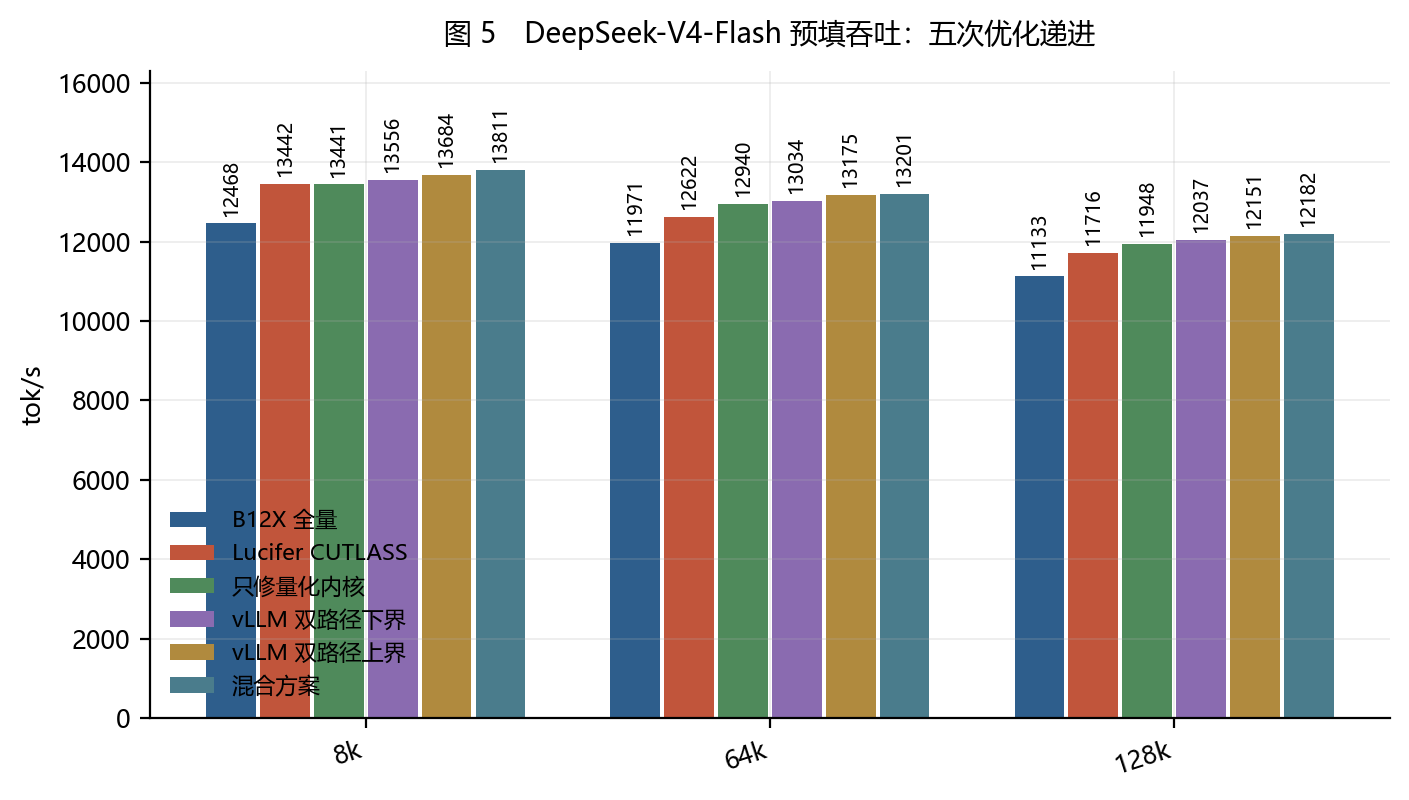
\includegraphics[width=0.86\textwidth]{../figures/fig-5.png}
\caption{图 5　DeepSeek-V4-Flash 预填吞吐：五次优化递进。}
\label{fig:8}
\end{figure*}

图 5 按优化次序排列，五次改动全部单调改善，没有任何一次回退。


同一台双卡 RTX PRO 6000 \textbf{WS}（TP2、force-A8 MoE、独立预填、\texttt{max\_num\_seqs=1}、fp8 KV、block 256）上，五个逐步改动的版本 {\scriptsize\texttt{c-\hspace{0pt}df-\hspace{0pt}rtx6k-\hspace{0pt}baseline}}：


\begin{table*}[t]
\centering
\footnotesize
\setlength{\tabcolsep}{4pt}
\label{tab:15}
\begin{tabular}{lrrrll}
\toprule
上下文 & B12X 全量 & Lucifer CUTLASS & 只修量化内核 & vLLM 双路径（区间） & 混合方案 \\
\midrule
8k & 12,468 & 13,442 & 13,441 & 13,556 至 13,684 & \textbf{13,811} \\
64k & 11,971 & 12,622 & 12,940 & 13,034 至 13,175 & \textbf{13,201} \\
128k & 11,133 & 11,716 & 11,948 & 12,037 至 12,151 & \textbf{12,182} \\
\bottomrule
\end{tabular}
\end{table*}

三个可读出的东西：


\textbf{其一，总收益稳定在 9\%-\hspace{0pt}11\%。} 8k 提升 \textbf{10.8\%}，128k 提升 \textbf{9.4\%}。


\textbf{其二，收益不来自单一改动。} 从 B12X 到 Lucifer CUTLASS 拿到 7.8\%（8k），再「只修量化内核」在 8k 上几乎是零（13,442 到 13,441），却在 64k 上拿到 2.5\%（12,622 到 12,940）。\textbf{同一改动在不同上下文长度上的收益不同。}


\textbf{其三，有一个改动是单调的。} 「+ vLLM 双路径」与「混合方案」在三档上都改善，而这是唯一一组在三档上都不倒退的改动。


\begin{quote}\small
\textbf{\sym{⭐}{}\sym{⭐}{} 判据}

当一个配置的收益随上下文长度变化时，「这个优化提升了 N\%」这句话必须带上下文长度才有意义。本报告在 8k 上说「+10.8\%」、在 128k 上说「+9.4\%」，\textbf{两者都是同一个改动的结果，但它们是两个数字}。

\end{quote}

\subsection{解码：在 300 W 档位上的横向位置}

\begin{figure*}[t]
\centering
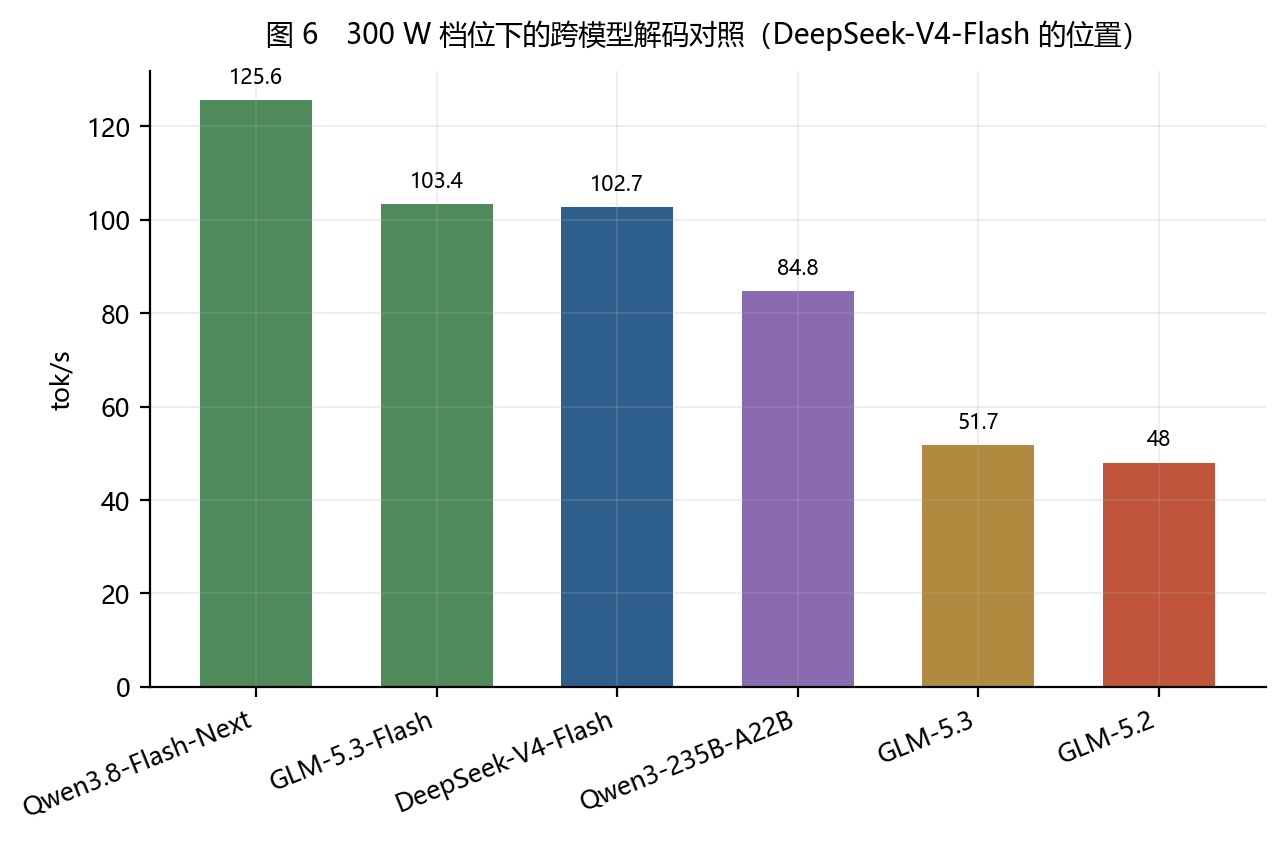
\includegraphics[width=0.86\textwidth]{../figures/fig-6.png}
\caption{图 6　300 W 档位下的跨模型解码对照。}
\label{fig:9}
\end{figure*}

图 6 的六根柱子都在同一功耗与同一上下文下测得，故它们之间的差异只反映模型本身。


单卡 300 W、pp2048 / tg128、单客户端下的一份跨模型表 {\scriptsize\texttt{c-\hspace{0pt}ds-\hspace{0pt}300w-\hspace{0pt}catalog}}：


\begin{table*}[t]
\centering
\footnotesize
\setlength{\tabcolsep}{4pt}
\label{tab:16}
\begin{tabular}{lll}
\toprule
模型 & 解码 tok/s & 预填 tok/s \\
\midrule
Qwen3.8-Flash-Next & \textbf{125.6} & 7,795 \\
GLM-5.3-Flash & 103.4 & \textbf{8,718} \\
\textbf{DeepSeek-V4-Flash} & \textbf{102.7} & 6,341 \\
Qwen3-235B-A22B & 84.8 & 4,808 \\
GLM-5.3 & 51.7 & 2,200 \\
GLM-5.2 & 48.0 & 2,197 \\
\bottomrule
\end{tabular}
\end{table*}

\textbf{DeepSeek-V4-Flash 在解码上排第三}，落后 Qwen3.8-Flash-Next \textbf{18.2\%}、落后 GLM-5.3-Flash \textbf{0.7\%}，领先 Qwen3-235B-A22B \textbf{21.1\%}。


\textbf{而它在预填上排第四}：6,341 落后 GLM-5.3-Flash \textbf{27.3\%}、落后 Qwen3.8-Flash-Next \textbf{18.7\%}。


\begin{quote}\small
\textbf{\sym{⭐}{}\sym{⭐}{}\sym{⭐}{} 一个反直觉的发现}

\textbf{同一个模型在解码榜和预填榜上的排名不同。}GLM-5.3-Flash 解码只比它快 0.7\%（在噪声内），预填却快 27.3\%。

故「A 模型比 B 模型快」这句话，\textbf{连「同一个模型」内部都不成立}：它取决于你问的是预填还是解码。

\end{quote}

\subsection{长上下文的真实代价：不是上下文，是输出长度}

\begin{figure*}[t]
\centering
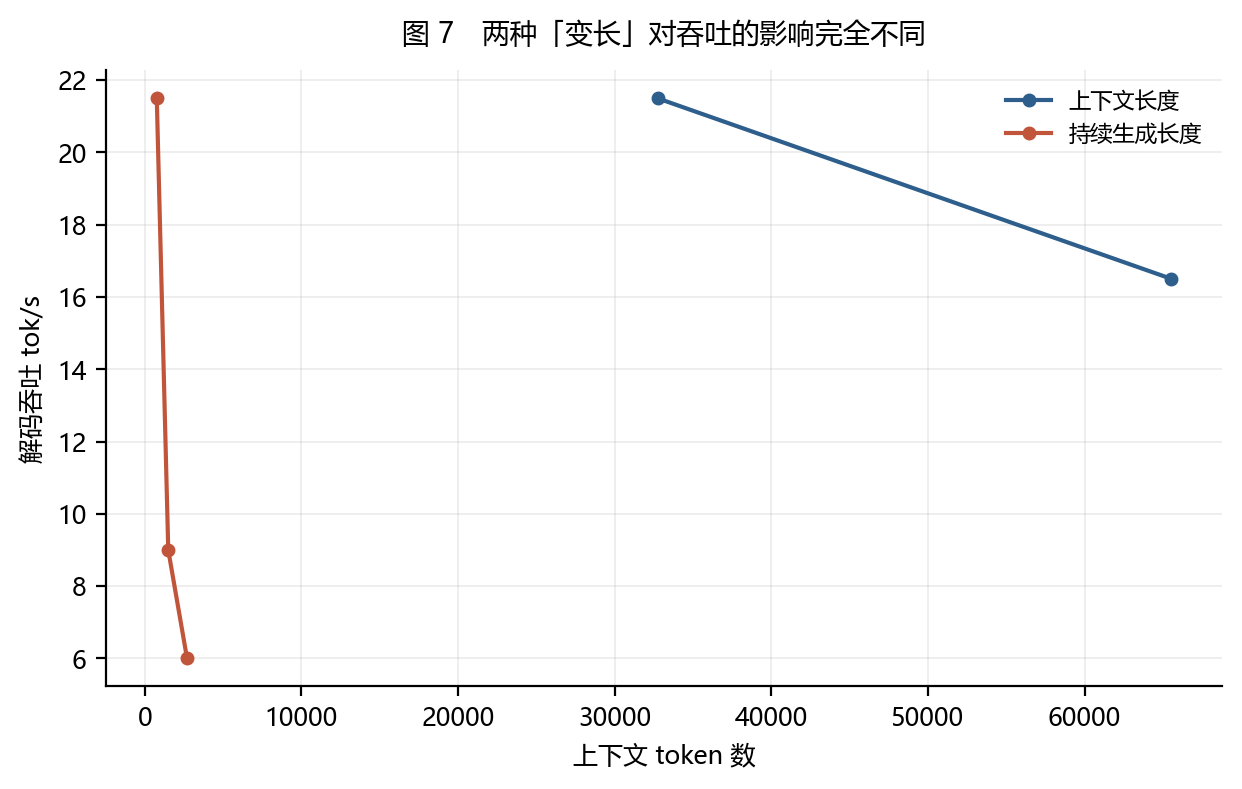
\includegraphics[width=0.86\textwidth]{../figures/fig-7.png}
\caption{图 7　两种「变长」对吞吐的影响完全不同。}
\label{fig:10}
\end{figure*}

图 7 的两条曲线一个缓慢下降、一个断崖下跌，这就是「长上下文慢」这个说法必须拆开的原因。


档案里有一条此前完全没有记录的性能现象，而它\textbf{不是关于上下文长度的} {\scriptsize\texttt{c-\hspace{0pt}long-\hspace{0pt}sustained-\hspace{0pt}gen-\hspace{0pt}degrades}}：


\begin{itemize}
  \item 32K 上下文、768-token 基准三次：19.97 / 21.18 / 23.31，\textbf{均值 21.49 tok/s}
  \item 64K 上下文、同样基准：\textbf{16-\hspace{0pt}17 tok/s}（降 \textbf{23\%}）
  \item 而通过 Open WebUI 流式做 \textbf{1,500-\hspace{0pt}2,700 token 的持续生成}时：\textbf{掉到约 6-\hspace{0pt}9 tok/s}
\end{itemize}

\textbf{降幅 58\%-\hspace{0pt}72\%，远大于上下文的 23\%。}


\begin{quote}\small
\textbf{\sym{⭐}{}\sym{⭐}{}\sym{⭐}{}\sym{⭐}{}\sym{⭐}{} 判据}

「长上下文慢」与「长输出慢」是两件事，而后者严重得多。而多数基准只测短输出的稳态解码，\textbf{于是这个现象在所有基准里都不可见}。

\textbf{故「tok/s」这个数必须带「生成多长」才有意义。}一个 21.49 tok/s 的基准成绩，与用户在对话里真实感受到的 6-\hspace{0pt}9 tok/s，差 3 倍，而两者测的是同一个模型、同一台机器。

\end{quote}

注意：这组数据的硬件是 \textbf{双 DGX Spark（2× GB10）}，不是 RTX PRO 6000。故它证明的是\textbf{模型行为}，不是这张卡的性能。但它对推理性能的意义是通用的。


\subsection{同条件对照：Spark 慢 6 倍，而差距不来自架构}

一条同条件对照给出了量级 {\scriptsize\texttt{c-\hspace{0pt}spark-\hspace{0pt}6x-\hspace{0pt}slower}}：2 张 DGX Spark 做 TP2，在 DeepSeek-V4-Flash 上比 2 张 RTX 6000 做 TP2 \textbf{慢约 6 倍}。


而两者共享同一批 SM120 核心。\textbf{故差距不来自架构，来自显存带宽与每卡功耗。}


\begin{quote}\small
\textbf{\sym{⭐}{}\sym{⭐}{} 判据}

这是本文最干净的一条「控制变量」证据：同一 compute capability、同一模型、同样 TP=2，\textbf{只换内存子系统与功耗预算}，结果差 6 倍。

故在推理场景里，\textbf{「架构代际」不是主要变量，带宽与功耗才是}。

\end{quote}

\subsection{百万上下文：可行，但瓶颈不是显存}

DeepSeek-V4-Flash 在 llama.cpp 上成功生成了第 \textbf{1,048,573} 个 token，即跑满 \textbf{1,048,576} 上下文 {\scriptsize\texttt{c-\hspace{0pt}1m-\hspace{0pt}feasible}}。


而档案里有两条互相印证的解释，说明\textbf{为什么只有它能做到}：


\textbf{其一，依赖模型结构。} 具备稀疏注意力 / indexer 的模型（正是 DeepSeek-V4-Flash）可以做到；而 MiMo V2.5 只是交替 SWA 与非 SWA 层，会尝试为完整上下文分配 KV，单次请求就要 \textbf{68,625 MiB} 而 OOM。


\textbf{其二，真实瓶颈是 32 位整数溢出。} 当 \texttt{n\_kv × n\_ubatch} 越过 2³² 边界时崩溃；具体边界是 \textbf{262,144 × 16,384 = 2³²}。修复方式是把 \texttt{flash\_attn\_mask\_to\_KV\_max} 的步长参数从 32 位 \texttt{int} 改为 64 位 \texttt{size\_t}，经第三方在相同设置下验证，处理 \textbf{334,585} 个新 token（约 1.5 小时）无崩溃。


\begin{quote}\small
\textbf{\sym{⚠}{}\sym{⚠}{}\sym{⚠}{} 判据}

「长上下文 OOM」这个诊断在 262,144 这个点上\textbf{是错的}：它不是显存不够，而是整数溢出。而这两者的表象完全相同（进程崩溃），故只能靠算那个乘法来区分。

\end{quote}

\subsection{而它在 SM120 上曾经完全跑不起来}

必须记录的一条：\textbf{纯上游 vLLM 在 SM120 上完全无法服务 DeepSeek-V4}，且被逐层剥离出\textbf{四个互相独立的阻塞点} {\scriptsize\texttt{c-\hspace{0pt}ds-\hspace{0pt}upstream-\hspace{0pt}cannot-\hspace{0pt}run}}。


其中最深的一个：mHC（Manifold-Constrained Hyper-Connections）层调用\texttt{tf32\_hc\_prenorm\_gemm}，而 DeepGEMM 树里只有 SM90 与 SM100 的实现——\texttt{sm100\_*} 用 TMEM / \texttt{tcgen05.mma} / cluster multicast，\texttt{sm90\_*} 用 WGMMA，\textbf{不存在 \texttt{sm120\_*} 变体}。报错发生在 \texttt{hyperconnection.hpp:56}。


而现场报告同时给出了一个乐观判断：SM120 原生支持 warp 级\texttt{mma.sync.aligned.m16n8k32}（SM80 时代）外加 TMA，故一个朴素移植「\textbf{在功能上是正确的……吞吐不是最优，但能解锁整个 V4 家族}」。


\begin{quote}\small
\textbf{\sym{⭐}{}\sym{⭐}{} 判据}

「这个模型能在 Blackwell 上跑」不是一个布尔值，而是一条\textbf{逐层清单}：权重加载、量化配置、MoE 分派、注意力后端、以及 mHC。前四项都过了，第五项断言失败。

\textbf{故「支持」这个词在没有清单的情况下没有信息量。}

\end{quote}



\section{96 GB 真正买到的是什么：上下文预算}

如果 96 GB 买的不是速度，那它买的是什么？本节给出可以算出来的答案。


\begin{figure*}[t]
\centering
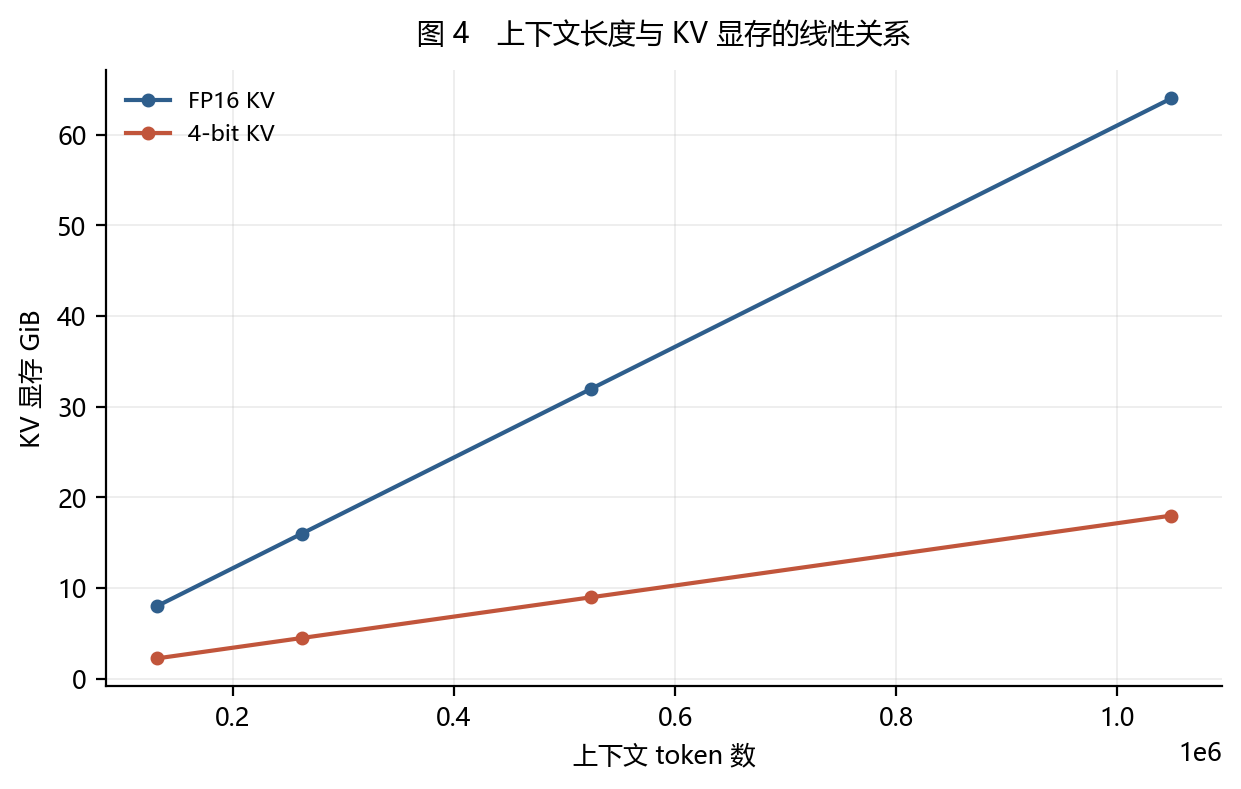
\includegraphics[width=0.86\textwidth]{../figures/fig-4.png}
\caption{图 4　上下文长度与 KV 显存的线性关系。}
\label{fig:11}
\end{figure*}

图 4 的直线斜率就是那个 18.3 KiB 的乘数，四条参考线分别对应四种精度的 KV 格式。


关键的乘数是\textbf{每 token 的 KV 字节数}。这个数在本报告里长期缺失——68 处「上下文 与 显存」的表述中，只有 1 处给了它。


两个独立来源给出了同一个值：


\begin{itemize}
  \item Bonsai 2 27B README：\textbf{FP16 KV cache 64 KiB per token}（100K ≈ 6.3 GiB）
  \item 本档案的压缩记录（见 §6）：\textbf{18.3 KiB/活跃 token、相对 BF16 3.50×} \sym{⇒}{} 18.3 × 3.50 = \textbf{64.05 KiB}
\end{itemize}

两者相差 \textbf{0.08\%} {\scriptsize\texttt{c-\hspace{0pt}two-\hspace{0pt}independent-\hspace{0pt}models-\hspace{0pt}agree-\hspace{0pt}on-\hspace{0pt}64-\hspace{0pt}kib-\hspace{0pt}per-\hspace{0pt}token}}。同一张表还给了「相对 FP8 1.75×」\sym{⇒}{} 18.3 × 1.75 = \textbf{32.02 KiB}，即 FP8 恰为 FP16 的一半。三个精度构成一条等比链：\textbf{FP16 64 / FP8 32 / 压缩 18.3 KiB}。


\begin{quote}\small
\textbf{\sym{⭐}{}\sym{⭐}{}\sym{⭐}{} 判据}

当一个常量由两个完全不同的模型（不同层数、不同头数）独立算出相同的值时，它说明的不是「这两个模型一样」，而是「这个量级被架构约束住了」。

\end{quote}

按 64 KiB/token 换算：


\begin{table*}[t]
\centering
\footnotesize
\setlength{\tabcolsep}{4pt}
\label{tab:17}
\begin{tabular}{rll}
\toprule
上下文 & FP16 KV & 4-bit KV（18 KiB） \\
\midrule
131,072 & \textbf{8.0 GiB} & 2.25 GiB \\
262,144 & \textbf{16.0 GiB} & 4.5 GiB \\
524,288 & \textbf{32.0 GiB} & 9.0 GiB \\
1,048,576 & \textbf{64.0 GiB} & 18.0 GiB \\
\bottomrule
\end{tabular}
\end{table*}

换算依据 {\scriptsize\texttt{c-\hspace{0pt}fp16-\hspace{0pt}kv-\hspace{0pt}cache-\hspace{0pt}is-\hspace{0pt}64-\hspace{0pt}kib-\hspace{0pt}per-\hspace{0pt}token}} {\scriptsize\texttt{c-\hspace{0pt}256k-\hspace{0pt}context-\hspace{0pt}costs-\hspace{0pt}16-\hspace{0pt}gib-\hspace{0pt}of-\hspace{0pt}kv}} {\scriptsize\texttt{c-\hspace{0pt}4bit-\hspace{0pt}kv-\hspace{0pt}cuts-\hspace{0pt}per-\hspace{0pt}token-\hspace{0pt}cost-\hspace{0pt}to-\hspace{0pt}18-\hspace{0pt}kib}}。


\textbf{这张表改变了三个此前说不清的问题。}


\textbf{其一，256K 上下文不是瓶颈。} 它只吃 16 GiB，在 96 GB 上占比不到 1/6。


\textbf{其二，1M 上下文才逼近上限。} 64 GiB 的 KV 之后只剩 32 GiB 装权重——于是问题从「显存够不够放 KV」变成「剩下的够不够放模型」。


\textbf{其三，KV 量化在这张卡上是一个「不需要」的优化。} 4-bit 在 1M 上省下 46 GiB，但那 46 GiB 在 96 GB 上并没有对应的瓶颈。


\begin{quote}\small
\textbf{\sym{⚠}{}\sym{⚠}{}\sym{⚠}{} 一条必须同时给出的限制}

「某模型能跑 N 上下文」这句话\textbf{不能跨模型迁移} {\scriptsize\texttt{c-\hspace{0pt}a-\hspace{0pt}context-\hspace{0pt}capability-\hspace{0pt}does-\hspace{0pt}not-\hspace{0pt}transfer-\hspace{0pt}between-\hspace{0pt}models}}。因为 显存占用 = 权重 + N × 每 token 字节数，而后一项由层数、KV 头数、头维度与 KV 精度共同决定。本文实测的两个模型就差 \textbf{3.5 倍}（64 vs 18.3 KiB）。

\textbf{故「这张卡支持 N 上下文」应一律改写为「在模型 M 上支持 N」。}

\end{quote}

这条限制的一个直接应用：本报告曾记有「单张，320K 上下文只用 44 GB 显存」。按 64 KiB/token 反推，320K 本身就要 \textbf{20.0 GiB} 的 KV，故余下约 24 GB 才是权重——\textbf{那是一个约 20 GB 权重的小模型的结果，不是这张卡的通用能力}。原文已在该处加注更正，旧文保留。



\section{五个让测量失效的陷阱}

本节记录的是\textbf{方法}，不是结论。它们全部来自这批资料的采集过程，每一条都曾造成过一个错误数字。


\subsection{HTTP 200 不等于拿到了内容}

抓取 TechPowerUp 的 \texttt{rtx-pro-6000.c4290} 返回 \textbf{HTTP 200}，响应体 \textbf{118,611 字符}——但 \texttt{<title>} 是「\textbf{AMD Radeon AI PRO R9700 Specs}」，且带 \texttt{noindex,nofollow}。正文纯文本只有 \textbf{335 字符}，搜「96 GB」\textbf{零命中}。


\begin{quote}\small
\textbf{判据}：当反爬策略选择「返回一张无关但完整的页面」时，它比 403 危险得多——因为 403 会让调用方停下来，而 200 会让它把无关内容当成答案。\textbf{故抓取日志的最小字段应是「状态码 + 标题 + 目标关键字命中数」三项。}

\end{quote}

\subsection{参数「存在但无效」}

Bonsai 的推理档位有 \texttt{xhigh} / \texttt{medium} / \texttt{low} 三档，但原文写着：\textbf{\texttt{low} 不被支持，选中时行为接近 \texttt{xhigh}} {\scriptsize\texttt{c-\hspace{0pt}xhigh-\hspace{0pt}is-\hspace{0pt}default-\hspace{0pt}and-\hspace{0pt}low-\hspace{0pt}is-\hspace{0pt}unsupported}}。


\begin{quote}\small
\textbf{判据}：当一个参数「存在但无效」时，它比「不存在」更危险——因为调用方会以为自己调低了成本，而实际行为与最高档相同。

\end{quote}

\subsection{能力数字缺少模型规模}

见 §5 末尾的 320K/44 GB 例子。同一个数字在加上模型规模前后是两条完全不同的结论。


\subsection{零提及的文档被整批跳过}

Bonsai README（24,840 字节）里 \texttt{RTX PRO} / \texttt{96 GB} / \texttt{5090} / \texttt{4090} 的出现次数\textbf{全是 0} {\scriptsize\texttt{c-\hspace{0pt}the-\hspace{0pt}bonsai-\hspace{0pt}readme-\hspace{0pt}has-\hspace{0pt}no-\hspace{0pt}pro-\hspace{0pt}6000-\hspace{0pt}data}}。按「是否提到目标硬件」筛选，它会被整个丢掉——而它恰恰是 §5 那个关键乘数的来源。


\begin{quote}\small
\textbf{判据}：读文档的目的不应只是「找数字」，还包括「找乘数」。

\end{quote}

\subsection{型号名当作配置名}

见 §1.1。这是本文新增的一节，也是这批资料里代价最高的一条：\textbf{227 条主张因此无法定位} {\scriptsize\texttt{c-\hspace{0pt}227-\hspace{0pt}of-\hspace{0pt}2233-\hspace{0pt}claims-\hspace{0pt}do-\hspace{0pt}not-\hspace{0pt}name-\hspace{0pt}a-\hspace{0pt}sku}}。



\subsection{五个陷阱的汇总}

<!-- tables/tab-2.md -->

\begin{table*}[t]
\centering
\footnotesize
\setlength{\tabcolsep}{4pt}
\caption{五个让测量失效的陷阱：表现、为何会骗人、如何识别。}
\label{tab:18}
\begin{tabularx}{\textwidth}{lXll}
\toprule
陷阱 & 表现 & 为何会骗人 & 如何识别 \\
\midrule
HTTP 200 诱饵页 & gpu-specs 返回 AMD R9700 页面 & 状态码正确但内容是另一个产品 & 校验标题是否含目标名 \\
参数存在但无效 & low 推理档等于 xhigh & 调用方以为降了成本 & 对比 low 与 xhigh 得到零差异 \\
能力数字无模型规模 & 320k 上下文只用 44 GB & 被读成显卡能力而非某模型结果 & 反推 KV 后看剩余权重 \\
零提及文档被跳过 & 25 KB README 无 PRO 6000 字样 & 丢掉了跨硬件通用的常量 & 按可否换算排序检索 \\
单位不可通约 & GPU-seconds 与 tok/s 并列 & 分母与所含项都不同 & 禁止同表比较 \\
\bottomrule
\end{tabularx}
\end{table*}



\section{渲染负载的对照：SKU 排序会反转}

\begin{figure*}[t]
\centering
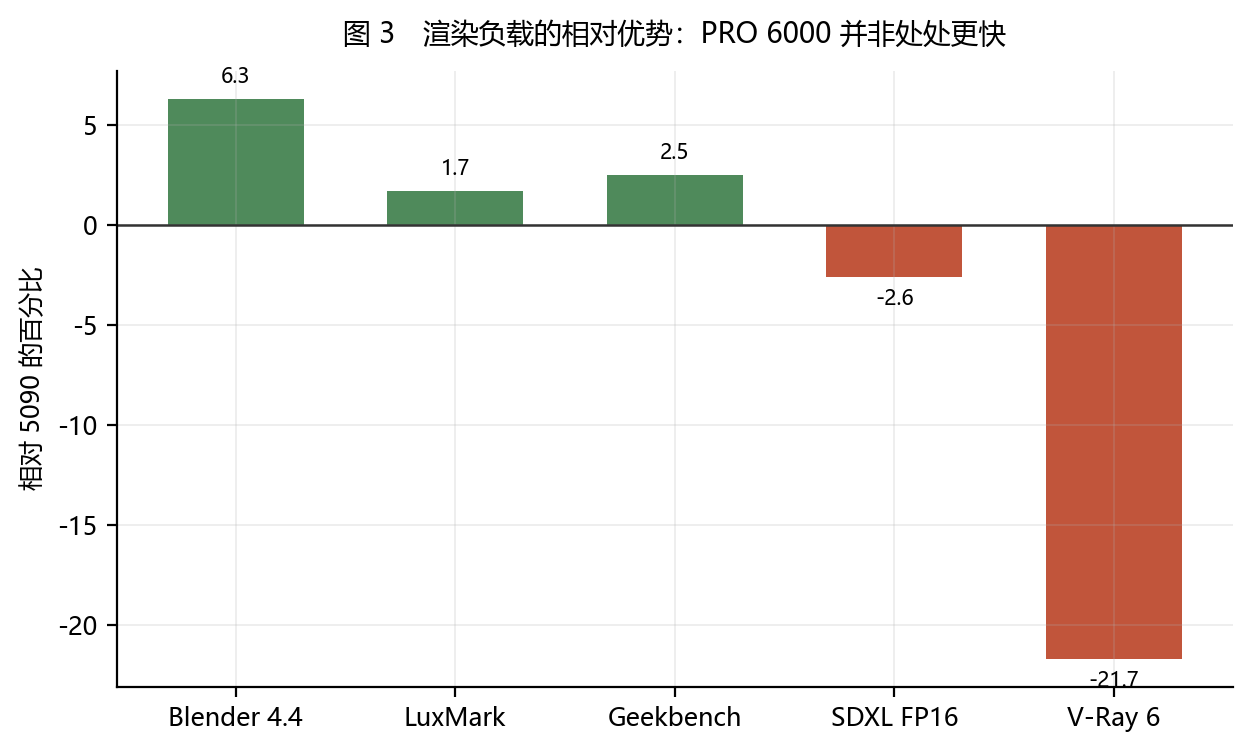
\includegraphics[width=0.86\textwidth]{../figures/fig-3.png}
\caption{图 3　渲染负载的相对优势：并非处处更快，且 SKU 排序会反转。}
\label{fig:12}
\end{figure*}

图 3 把六个渲染器的相对优势画在同一尺度上，正负号的分界正是「谁更快」这个问题的答案分裂处。


\begin{table*}[t]
\centering
\footnotesize
\setlength{\tabcolsep}{4pt}
\label{tab:19}
\begin{tabularx}{\textwidth}{lX}
\toprule
负载 & 相对 RTX 5090 \\
\midrule
Blender 4.4（\texttt{WS}，三场景均值） & \textbf{+6.3\%} \\
LuxMark（\texttt{WS}） & \textbf{+1.7\% \textasciitilde{} +5.0\%}（claim 记下限/上限） \\
Geekbench（\texttt{WS}） & \textbf{+2.5\%} \\
SDXL FP16（\texttt{WS}） & \textbf{-2.6\%} \\
V-Ray 6（\texttt{WS}，vpaths） & \textbf{-21.7\%} \\
\bottomrule
\end{tabularx}
\end{table*}

数据来源 {\scriptsize\texttt{c-\hspace{0pt}sr-\hspace{0pt}renderer-\hspace{0pt}split}} {\scriptsize\texttt{c-\hspace{0pt}sr-\hspace{0pt}blender-\hspace{0pt}narrow}} {\scriptsize\texttt{c-\hspace{0pt}sr-\hspace{0pt}vray-\hspace{0pt}loses}}。


V-Ray 6 上 RTX 5090 以 14,764 vpaths 领先 \texttt{WS} 版的 12,128 {\scriptsize\texttt{c-\hspace{0pt}sr-\hspace{0pt}vray-\hspace{0pt}loses}}。


\textbf{而 SKU 排序在这里也反转了} {\scriptsize\texttt{c-\hspace{0pt}sku-\hspace{0pt}order-\hspace{0pt}inverts-\hspace{0pt}between-\hspace{0pt}renderers}}：


\begin{table*}[t]
\centering
\footnotesize
\setlength{\tabcolsep}{4pt}
\label{tab:20}
\begin{tabular}{lllrrl}
\toprule
基准 & WS & Server & Max-Q & 5090 & 结论 \\
\midrule
Blender Open Data & 18,571 & 18,580 & 18,678 & 18,747 & \textbf{四者极差 0.9\%} \\
OctaneBench 2025.2 & \textbf{1750} & 1641 & 1601 & — & WS > SE > MQ \\
V-Ray 6 & 11,994 & \textbf{14,827} & — & 10,116 & \textbf{SE 反超 WS 23.6\%} \\
\bottomrule
\end{tabular}
\end{table*}

\begin{quote}\small
\textbf{\sym{⭐}{}\sym{⭐}{}\sym{⭐}{}\sym{⭐}{}\sym{⭐}{} 判据}

当同一批 SKU 在三个基准上给出\textbf{三种排序}时，「哪个 SKU 更快」这个问题本身没有答案——只有「在哪个基准上更快」有答案。

\textbf{故凡见「A 版比 B 版快」，必须同时给出基准名与差值，缺一不可。}

\end{quote}

而 §4 那个 928\% 与这里的 -21.7\% 并存，说明：\textbf{这张卡的价值曲线不是「更快」，而是「在容量边界附近突然可用」。}



\section{能耗与成本：买得起不等于用得起}

这一章要回答的是最实际的一问：\textbf{值不值得买。}而它会给出一个自我矛盾的答案——\textbf{八个指标里，这张卡赢两个、输六个。}


\subsection{按芯片成本排，它最便宜}

\begin{figure*}[t]
\centering
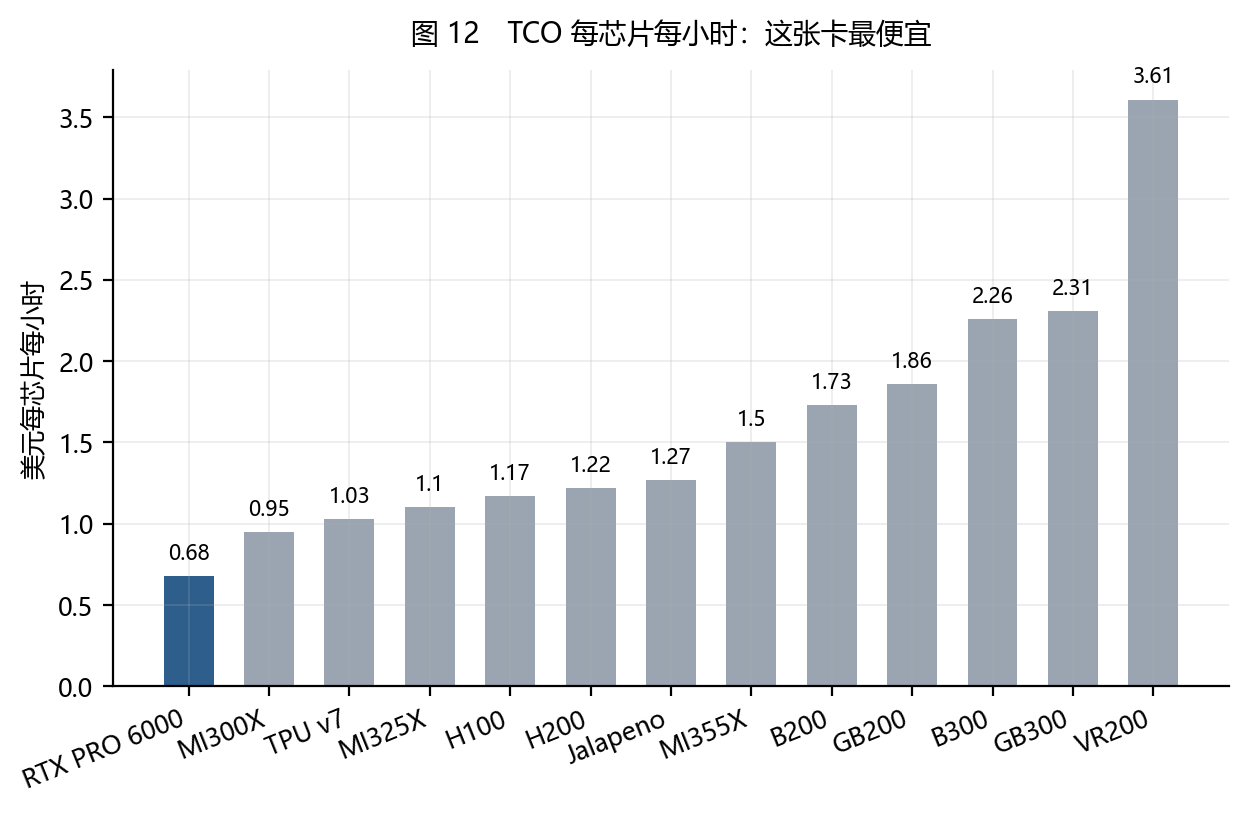
\includegraphics[width=0.86\textwidth]{../figures/fig-12.png}
\caption{图 12　TCO 每芯片每小时：这张卡最便宜。}
\label{fig:13}
\end{figure*}

图 12 按 TCO 每芯片每小时排列 13 张加速器，\textbf{RTX PRO 6000 的 0.68 美元最低}，是 GB300 的 2.31 美元的 \textbf{29\%}——便宜 3.4 倍 {\scriptsize\texttt{c-\hspace{0pt}ix-\hspace{0pt}paradox}}。


\sym{⚠}{} 注意这一维\textbf{越低越好}，而它是本文唯一一张「本卡领先」的成本图。


\subsection{按 token 成本排，它最贵}

\begin{figure*}[t]
\centering
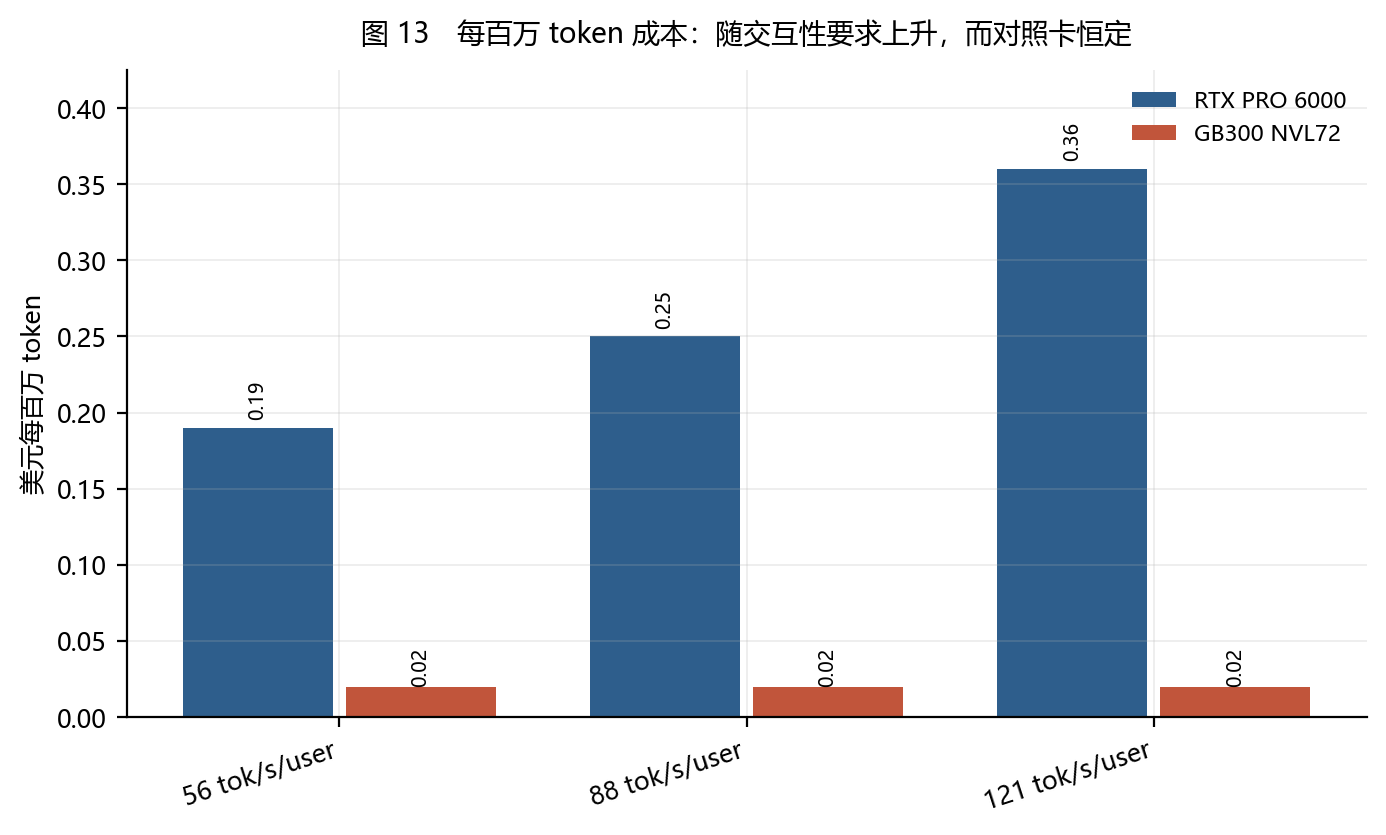
\includegraphics[width=0.86\textwidth]{../figures/fig-13.png}
\caption{图 13　每百万 token 成本：随交互性要求上升，而对照卡恒定。}
\label{fig:14}
\end{figure*}

\begin{table*}[t]
\centering
\footnotesize
\setlength{\tabcolsep}{4pt}
\caption{买得起不等于用得起：每芯片成本与每百万 token 成本。}
\label{tab:21}
\begin{tabular}{lrll}
\toprule
芯片 & 每芯片每小时成本（美元） & 每百万 token 成本（美元） & 该交互性下的并发数 \\
\midrule
RTX PRO 6000 & 0.68 & 0.19 & 10 \\
MI325X & 1.1 & 未给出 & 未给出 \\
H100 & 1.17 & 未给出 & 未给出 \\
H200 & 1.22 & 未给出 & 未给出 \\
B200 & 1.73 & 未给出 & 未给出 \\
GB300 & 2.31 & 0.02 & 约 2983 \\
\bottomrule
\end{tabular}
\end{table*}
按芯片逐行对照，可以看到「每芯片每小时」这一列它最低，而「每百万 token」这一列只有对照卡给了数、且相差一个量级。


图 13 把三组柱子并排，可以看到对照卡的三根完全等高，而这张卡的三根逐级抬升。


同一份来源、同一个模型（Qwen 3.5 397B-A17B）、同一精度（FP4），目标交互性从 56 提到 121 tok/s/user 时 {\scriptsize\texttt{c-\hspace{0pt}ix-\hspace{0pt}perdollar}}：


\begin{itemize}
  \item \textbf{RTX PRO 6000}：\$0.19 \sym{→}{} \$0.25 \sym{→}{} \$0.36 每百万 token
  \item \textbf{GB300 NVL72}：\$0.02 \sym{→}{} \$0.02 \sym{→}{} \$0.02
\end{itemize}

\textbf{对照卡的成本是平的，而这张卡随要求变高而上涨。}


原因是并发：同一交互性点（56 tok/s/user）下，GB300 NVL72 能同时服务约 \textbf{2,983} 路请求，而这张卡约 \textbf{10} 路 {\scriptsize\texttt{c-\hspace{0pt}ix-\hspace{0pt}paradox}}。


\begin{quote}\small
\textbf{\sym{⭐}{}\sym{⭐}{}\sym{⭐}{}\sym{⭐}{}\sym{⭐}{} 判据（本文第二条）}

\textbf{低芯片成本无法弥补低并发。}

一张便宜 3.4 倍的卡，若每单位时间能卖出的 token 少 298 倍，那么它的单位 token 成本会贵 9.5 倍。\textbf{「买得起」与「用得起」是两个完全不同的判据，且方向相反。}

\end{quote}

\begin{table*}[t]
\centering
\footnotesize
\setlength{\tabcolsep}{4pt}
\caption{六个成本与能效指标，指向不同的卡。}
\label{tab:22}
\begin{tabular}{lllll}
\toprule
指标 & RTX PRO 6000 & 对照卡 & 谁更优 & 口径 \\
\midrule
TCO 美元每芯片每小时 & 0.68 & GB300 为 2.31 & RTX 为 29\% 即便宜 3.4 倍 & 来源直接给出 \\
每百万 token 成本 56 tok/s & 0.19 美元 & GB300 为 0.02 美元 & GB300 更省 & 来源直接给出 \\
每百万 token 成本 121 tok/s & 0.36 美元 & GB300 为 0.02 美元 & GB300 更省 & 来源直接给出 \\
成本效率差距 56 tok/s & 1.0 & 高出 1047\% & GB300 更优 & 来源原话 \\
同交互性下并发 56 tok/s & 约 10 & GB300 约 2983 & GB300 高约 298 倍 & 来源直接给出 \\
每美元性能 & 领先 2.1 倍 & 落后 & H100 NVL 为参照 & 来源直接给出 \\
每瓦性能 & 落后约 1.5 倍 & 领先 & H100 为参照 & 来源直接给出 \\
单卡总能耗 SDXL & 1.35 Wh & 5090 为 1.16 Wh & 5090 略优 & 来源直接给出 \\
\bottomrule
\end{tabular}
\end{table*}

\subsection{一处必须如实写出的口径差异}

来源对 56 tok/s/user 这一点的原话是「GB300 NVL72 的成本效率高出 \textbf{1047\%}」{\scriptsize\texttt{c-\hspace{0pt}ix-\hspace{0pt}perdollar}}。


而按两数直接相除：0.19 除以 0.02 再减 1，等于 \textbf{850\%}。


\textbf{1047\% 对应 11.47 倍，850\% 对应 9.5 倍。} 两者差 20\%。


\begin{quote}\small
\textbf{\sym{⭐}{}\sym{⭐}{}\sym{⭐}{} 判据}

「成本效率」这个词有多种口径：可以是成本之比，也可以是「同样预算能买到多少 token」，中间可能含别的时间折算。而来源没有展开它是哪一种。

\textbf{本文两个数都写，并注明哪个是来源的、哪个是我按两数算的。}把不吻合的地方隐去，比算错更糟——因为下一个人会以为它对得上。

\end{quote}

\subsection{能效：另一个方向相反的指标}

在 SPECworkstation 类负载上（\texttt{WS} 版），整机平均功耗 \textbf{918.5 W}、峰值 \textbf{1,036.3 W}、空闲 152.3 W；SDXL FP16 的 5.3 秒测试区间总能耗 \textbf{1.35 Wh} {\scriptsize\texttt{c-\hspace{0pt}sr-\hspace{0pt}power-\hspace{0pt}918w}}。


\begin{table*}[t]
\centering
\footnotesize
\setlength{\tabcolsep}{4pt}
\label{tab:23}
\begin{tabular}{ll}
\toprule
卡 & 同负载总能耗 \\
\midrule
RTX PRO 6000 \texttt{WS} & \textbf{1.35 Wh} \\
RTX 4090 & \textbf{1.35 Wh} \\
RTX 5090 & 1.16 Wh \\
RTX 6000 Ada & 1.76 Wh \\
\bottomrule
\end{tabular}
\end{table*}

评测方指出，同为 GB202 芯片\textbf{且不同 SKU} 的新 Blackwell 卡在该负载下能效特征非常接近，\textbf{能耗差异主要来自 TDP 差异} {\scriptsize\texttt{c-\hspace{0pt}sr-\hspace{0pt}power-\hspace{0pt}converged}}。


而放到机架密度上看，方向又反了一次：\textbf{H100 约 1.5 倍性能每瓦} {\scriptsize\texttt{c-\hspace{0pt}slac-\hspace{0pt}power-\hspace{0pt}favors-\hspace{0pt}h100}}。


\begin{quote}\small
\textbf{\sym{⭐}{}\sym{⭐}{}\sym{⭐}{} 判据}

于是同一张卡在三个指标上分别排第一、倒数第一、和倒数第二：\textbf{每芯片成本最低、每 token 成本最高、每瓦性能落后 1.5 倍。}三者都是真的，选哪个取决于你的约束是资本、是吞吐、还是电。

\end{quote}

\subsection{价格本身也是一个陷阱}

价格必须按 SKU 分开记 {\scriptsize\texttt{c-\hspace{0pt}sr-\hspace{0pt}price-\hspace{0pt}8500}}：\texttt{WS} 首发 \textbf{\$8,500}，当前街价 \textbf{\$17,999}——两者相差一倍以上，而方向与「首发价 vs 一年后街价」相反，故更可能是两个来源采集口径不同（首发建议价 vs 稀缺期市场价），而不是价格真的上涨了一倍。


\begin{quote}\small
\textbf{\sym{⭐}{}\sym{⭐}{} 判据}

当两个来源对同一商品给出相反方向的价格差时，先怀疑口径，再怀疑市场。

\end{quote}



\section{结论与未解问题}

\subsection{结论}

\textbf{1. 「这张卡多快」不是一个问题，是三个问题。}预填 4,757 tok/s、解码 43.16 tok/s、首字延迟 673 毫秒，是同卡同模型同测量的三个数，前两者差 110 倍；而首字与吞吐的排序还会在不同的卡之间翻转：2 张 B200 吞吐高 1.66 倍、TPOT 低 2.3 倍，首字却慢 3.7 倍 {\scriptsize\texttt{c-\hspace{0pt}llamacpp-\hspace{0pt}prefill}}{\scriptsize\texttt{c-\hspace{0pt}llamacpp-\hspace{0pt}decode-\hspace{0pt}parity}}{\scriptsize\texttt{c-\hspace{0pt}ep-\hspace{0pt}ttft}}{\scriptsize\texttt{c-\hspace{0pt}ep-\hspace{0pt}gap}}。前者受算力限制、后者受带宽限制，故任何单点「加速比」都必须注明是哪一半。


\textbf{2. 这个产品名不是一个配置，而是三个。} 同一模型同一命令下 \texttt{MQ} 比 \texttt{WS} 慢 \textbf{12.9\%-\hspace{0pt}13.1\%}；同功耗点 300 W 上 \texttt{SE} 比 \texttt{WS} 快 \textbf{38\%} {\scriptsize\texttt{c-\hspace{0pt}sku-\hspace{0pt}choice-\hspace{0pt}changes-\hspace{0pt}tok-\hspace{0pt}s-\hspace{0pt}by-\hspace{0pt}13pct}}。而「比 5090 快还是慢」的答案随之翻转：\texttt{WS} 快 5\%，\texttt{MQ} 慢 12\%。


\textbf{3. 这张卡买的不是速度。} 容量不受约束时，\texttt{WS} 与 RTX 5090 的 token 速率差距只有 1.5\%-\hspace{0pt}5.9\% {\scriptsize\texttt{c-\hspace{0pt}sr-\hspace{0pt}token-\hspace{0pt}vs-\hspace{0pt}score}}。


\textbf{4. 它买的是「在容量边界上仍然可用」。} 120B 模型上 5090 无法加载，而它以 163.15 tok/s 完成 {\scriptsize\texttt{c-\hspace{0pt}sr-\hspace{0pt}96gb-\hspace{0pt}unique}}。这个差异的性质是可行性，不是速度。


\textbf{5. 96 GB 的实际形态是上下文预算。} 按 64 KiB/token，256K 需 16 GiB、1M 需 64 GiB {\scriptsize\texttt{c-\hspace{0pt}256k-\hspace{0pt}context-\hspace{0pt}costs-\hspace{0pt}16-\hspace{0pt}gib-\hspace{0pt}of-\hspace{0pt}kv}}。\textbf{后者的约束不是 KV 而是剩余权重空间。}


\textbf{6. 「买得起」与「用得起」方向相反，而两个数都是真的。}TCO 每芯片每小时 0.68 美元，13 张加速器里最低，是 GB300 的 29\%；但每百万 token 成本 0.19 到 0.36 美元，而 GB300 NVL72 三档恒为 0.02。原因不是性价比，是并发：同交互性下 GB300 服务约 2,983 路、这张卡约 10 路 {\scriptsize\texttt{c-\hspace{0pt}ix-\hspace{0pt}paradox}}{\scriptsize\texttt{c-\hspace{0pt}ix-\hspace{0pt}perdollar}}。\textbf{低芯片成本无法弥补低并发。}


\textbf{7. 渲染领域的结论不可外推，且 SKU 排序在基准间反转。} \texttt{SE} 在 V-Ray 上领先 \texttt{WS} 23.6\%，在 OctaneBench 上落后 6.2\%，在 Blender 上与 5090 打平 {\scriptsize\texttt{c-\hspace{0pt}sku-\hspace{0pt}order-\hspace{0pt}inverts-\hspace{0pt}between-\hspace{0pt}renderers}}。


\textbf{8. 「比上代提升 N 倍」这句话，选不同的基线可以差 20 倍。}对 L40 Ada 的实测中位是 1.09 倍、最差 0.85 倍；对同一对卡的厂商宣称最高是 5.6 倍；L2 缓存相对 RTX A6000 是 21.3 倍 {\scriptsize\texttt{c-\hspace{0pt}omni3-\hspace{0pt}vs-\hspace{0pt}l40-\hspace{0pt}median}}{\scriptsize\texttt{c-\hspace{0pt}vgpu-\hspace{0pt}l40s-\hspace{0pt}56}}{\scriptsize\texttt{c-\hspace{0pt}l2-\hspace{0pt}cache}}。故采购判据不能是「最高加速比」，必须是\textbf{你自己负载上的中位数}。


\textbf{9. 「与 H100 比」不是一个问题，是四个问题。} 每美元性能赢（便宜 2.1 倍）、每瓦性能输（落后约 1.5 倍）、每 token 成本大输（差约 9.5 倍）、单流解码输（带宽差 1.87 倍）。四个指标指向不同的结论 {\scriptsize\texttt{c-\hspace{0pt}slac-\hspace{0pt}h100-\hspace{0pt}vs-\hspace{0pt}rtx}}{\scriptsize\texttt{c-\hspace{0pt}slac-\hspace{0pt}power-\hspace{0pt}favors-\hspace{0pt}h100}}{\scriptsize\texttt{c-\hspace{0pt}ix-\hspace{0pt}paradox}}{\scriptsize\texttt{c-\hspace{0pt}hbm-\hspace{0pt}bw-\hspace{0pt}gap}}。故本文不给「谁更好」的排名，只给「在哪个约束下更好」。


\textbf{10. 同一个模型在预填榜与解码榜上的排名不同。} DeepSeek-V4-Flash 在 300 W 档的解码上排第三（102.7 tok/s，落后第一名 18.2\%），但在预填上排第四（6,341 tok/s，落后第一名 27.3\%）{\scriptsize\texttt{c-\hspace{0pt}ds-\hspace{0pt}300w-\hspace{0pt}catalog}}。故「A 模型比 B 模型快」这句话，连「同一个模型」内部都要先问是预填还是解码。


\textbf{11. 「长输出慢」比「长上下文慢」严重得多。} 上下文 32K 到 64K 只降 23\%，而持续生成从 768 token 拉到 1,500-2,700 token 会掉到 6-9 tok/s，降幅 58\%-72\%{\scriptsize\texttt{c-\hspace{0pt}long-\hspace{0pt}sustained-\hspace{0pt}gen-\hspace{0pt}degrades}}。而多数基准只测短输出，故这个现象在基准里不可见。


\textbf{12. 全部数字最高只到「测量级」。} 本文没有一条结论达到复现级——因为没有任何一条曾在第二台机器、同一 SKU 上被独立重测。


\subsection{未解问题}

\begin{table*}[t]
\centering
\footnotesize
\setlength{\tabcolsep}{4pt}
\label{tab:24}
\begin{tabularx}{\textwidth}{rXl}
\toprule
\# & 问题 & 类别 \\
\midrule
1 & §3、§4 两组基准数据的确切 SKU（来源未写明） & recoverable \\
2 & 未打补丁的原版 \texttt{llama.cpp} 在同一 SKU 上的数字 & recoverable \\
3 & SGLang 用 vLLM 那套参数在同一批 4 卡上的结果 & recoverable \\
4 & \texttt{llama-bench -r 3} 是否把受预热污染的第一轮算进平均 & recoverable \\
5 & 官方 Known Issue「multi-GPU on RTX Pro 6000」的具体内容 & context \\
6 & 同一量化在 \texttt{sm\_120} 与 \texttt{sm\_100} 上的成对对照 & context \\
\bottomrule
\end{tabularx}
\end{table*}

\begin{quote}\small
\textbf{\sym{⭐}{} 一个已经修掉的结构性缺陷}

上一版本文的 SKU 纪律是\textbf{事后加的散文}——227 条旧主张不带 SKU 字段。本轮把它变成了字段：\texttt{claims.csv} 新增 \texttt{sku} 列，校验器每次运行都报告\texttt{sku\_unspecified} 的当前值（现为 \textbf{244}）。

关键差别不在「多了一列」，而在\textbf{这个数字从此会出现在每次通过的输出里}：它无法再被忘记，也无法在无人察觉的情况下变大。

\end{quote}


\section{附录 A　证据等级说明}

\begin{table*}[t]
\centering
\footnotesize
\setlength{\tabcolsep}{4pt}
\label{tab:25}
\begin{tabular}{lll}
\toprule
级别 & 含义 & 本文中的数量 \\
\midrule
\texttt{untested} & 只是计划，没有执行 & 0 \\
\texttt{diagnostic} & 执行了，但用于诊断而非定论 & 部分 \\
\texttt{measured} & 有可追溯的测量记录 & \textbf{全部数值} \\
\texttt{reproduced} & 在独立环境被第二次测到 & \textbf{0} \\
\texttt{released} & 随产品发布并接受外部核验 & \textbf{0} \\
\bottomrule
\end{tabular}
\end{table*}

\section{附录 B　可复现性}

本文全部图表由 \texttt{scripts/render\_paper.py} 从 \texttt{paper/data/*.csv} 生成。每个数据行都有一列 \texttt{cite}，指向 \texttt{research/rtx-pro-6000/claims.csv} 里一个已存在的主张；渲染器在生成前会校验这些引用，缺一条就拒绝出图。


\begin{lstlisting}
python scripts/render_paper.py research/rtx-pro-6000/paper --check
python scripts/render_paper.py research/rtx-pro-6000/paper
python scripts/audit_paper.py research/rtx-pro-6000/paper
\end{lstlisting}

本文不新增任何事实。凡需要推导的数字，推导过程已作为 \texttt{derivation} 字段写在对应主张上。



\section{附录 C　本文与档案报告的关系}

本目录下有两份长文档，相差 \textbf{51 倍}：


\begin{table*}[t]
\centering
\footnotesize
\setlength{\tabcolsep}{4pt}
\label{tab:26}
\begin{tabular}{lll}
\toprule
 & \texttt{PAPER.md} / \texttt{PAPER.pdf} & \texttt{REPORT.md} \\
\midrule
规模 & 33,539 字符 & 1,694,296 字符 \\
结构 & 10 章、25 节、13 图、8 表 & 689 个顶层节（编号 1 到 692） \\
性质 & \textbf{综述}：已收敛的判断 & \textbf{工作档案}：逐轮的发现与失败记录 \\
读者 & 想知道结论的人 & 想核对过程、或接手这项工作的人 \\
是否自足 & 是，可独立阅读 & 否，需配合 \texttt{claims.csv} 使用 \\
\bottomrule
\end{tabular}
\end{table*}

\begin{quote}\small
\textbf{\sym{⭐}{}\sym{⭐}{}\sym{⭐}{} 一句话分工}

\textbf{\texttt{REPORT.md} 记录「我怎么知道的」，\texttt{PAPER.md} 给出「我知道什么」。}

前者按\textbf{时间}组织（第 N 轮查了什么），后者按\textbf{论证}组织（这个问题该用什么证据回答）。

\end{quote}

\sym{⚠}{} 档案的顶层节编号是 1 到 692 而有 689 个节，缺 15、258、261 三个号。那三节在早期版本里被合并了，编号没有回收。\textbf{这个缺口故意留着}：它让「某条结论是第几轮加的」可以被精确定位，回收编号会让旧的引用全部失效。


\subsection{为什么不合成一份}

两份文档的组织轴不同，合并必然牺牲其中一轴：


\begin{itemize}
  \item 按时间组织，读者要读完 689 节才知道结论是什么；
  \item 按论证组织，读者看不到「这条结论是怎么被推翻又重建的」。
\end{itemize}

而后者恰恰是这份工作最该保留的部分——\textbf{本文有 9 条主张标为 \texttt{disputed}，它们的价值不亚于成立的结论}，因为下一个人会遇到同样的分歧。


\subsection{两份文档如何保持同步}

\textbf{单向同步：档案是唯一的真相源，论文只能引用它。}


具体机制：


\begin{enumerate}
  \item 论文里每个数字后面挂一个方括号标记（形如 c- 加主张名），指向 \texttt{claims.csv} 的一个主张；
  \item \texttt{audit\_paper.py} 检查每个这样的标记都存在，且论文里的数值能在该主张的证据里找到；
  \item 图表的数据文件每行有 \texttt{cite} 列，\texttt{render\_paper.py} 出图前校验；
  \item 论文若引入档案里没有的数字，第 2 步直接失败。
\end{enumerate}

\textbf{故论文不可能包含档案里没有的事实。} 这条约束是机器强制的，不靠作者自觉。


\subsection{读者该怎么用}

\begin{itemize}
  \item \textbf{只想知道买不买}：读 §3.4（预填解码之别）与 §9（成本悖论）两节，约 8 页。
  \item \textbf{要选型}：读 §1（SKU 与容量两个前置问题）到 §6，约 18 页。
  \item \textbf{要核对某个数字}：在该数字后找那个方括号标记，到 \texttt{claims.csv} 查该行，
\end{itemize}
  再按 \texttt{evidence\_ids} 到 \texttt{evidence.csv} 取原文引用。三级可追。

\begin{itemize}
  \item \textbf{要接手这项工作}：读 \texttt{REPORT.md} 最后 30 节（§10.666 之后），
\end{itemize}
  那里是最近三轮的完整思路；再读 \texttt{scripts/README.md} 了解四道校验。


\subsection{已知的不一致，以及为什么留着}

本文正文与档案之间存在\textbf{两处口径差异}，都已在正文里标注：


\begin{enumerate}
  \item \textbf{成本效率 1047\% 对 850\%}（§9.3）：来源原话与按两数相除的结果差 20\%
\end{enumerate}
   而来源未展开口径；

\begin{enumerate}
  \item \textbf{SKU 未指明 244 条}（§1.1.4）：档案里 2,238 条主张中有 244 条无法定位 SKU，
\end{enumerate}
   本文引用的 46 条里有 17 条同样无法定位。


\begin{quote}\small
\textbf{\sym{⭐}{}\sym{⭐}{} 判据}

这两处都\textbf{不是等待修正的错误，而是等待更多来源的空白}。把它们抹平（比如取中间值、或按最可能的 SKU 归类）会让论文更整洁，也会让它更不可信。

\end{quote}



\end{document}
